\documentclass[a4paper,11pt]{article}
\pdfoutput=1
\usepackage{jheppub}
\usepackage{xcolor}
\colorlet{mdtRed}{red!50!black}
% \usepackage[]{hyperref}
\hypersetup{colorlinks=true,% Set to false to disable coloring links
% citecolor=mdtRed,% The color of citations
linkcolor=gray,% The color of references to document elements (sections, figures, etc)
urlcolor=mdtRed
}
\usepackage[utf8]{inputenc}

\usepackage{fancybox}
%\usepackage{cite}
\usepackage{float}
\usepackage{amsfonts}
\usepackage{amsmath}
\usepackage{amsbsy}
\usepackage{graphicx}
\usepackage{amssymb}
\usepackage{amsthm}
\usepackage{bm}
\usepackage{comment}
\usepackage{epsfig}
\usepackage{latexsym}
\usepackage{pdflscape}
\usepackage{color}
%\usepackage{collref}
%\usepackage{showkeys}
\usepackage{slashed}
\usepackage{tikz}
\usetikzlibrary{arrows.meta,decorations.markings}

\tikzset{
  mid arrow/.style={
    postaction={
      decorate,
      decoration={
        markings,
        mark=at position 0.5 with {\arrow{Stealth[length=6pt,width=6pt]}}
      }
    }
  }
}

\usepackage{cancel}
\usepackage{xcolor}
\usepackage{braket}
\usepackage{empheq}
\usepackage{graphicx} % Allows including images
\usepackage{braket}
\usepackage{tikz}
\usepackage{tikz-3dplot}
% réglage de la vue 3D : élévation=20°, azimut=110°
\tdplotsetmaincoords{20}{110}
\usetikzlibrary{decorations.pathreplacing,calc}
\usetikzlibrary{decorations.pathmorphing}
\usepackage{subcaption}
\usepackage{setspace}

\definecolor{blue5}{rgb}{0, 0, 0.66666}
\definecolor{red4}{rgb}{0.8, 0, 0}
\definecolor{navyblue}{rgb}{0, 0.2745, 0.67843}
\definecolor{cornflowerblue}{rgb}{0.388235, 0.6941176, 0.898039}
\usetikzlibrary{decorations.text,decorations.pathmorphing}

%Removes Header------------------------------------
\makeatletter
\def\@fpheader{\relax}
\makeatother



\usepackage{orcidlink}

%\DeclareMathOperator{\tr}{tr}
\DeclareMathOperator{\pf}{pf}
\DeclareMathOperator{\Ai}{Ai}
\DeclareMathOperator{\vol}{vol}
\DeclareMathOperator{\sgn}{sgn}
\DeclareMathOperator{\sn}{sn}
\DeclareMathOperator{\cn}{cn}
\DeclareMathOperator{\dn}{dn}
\DeclareMathOperator{\cd}{cd}
\DeclareMathOperator{\Det}{Det}
% \DeclareMathOperator{\tr}{tr}

\newcommand{\beq}{\begin{eqnarray}}
\newcommand{\eeq}{\end{eqnarray}}
\newcommand{\bea}{\begin{eqnarray}}
\newcommand{\eea}{\end{eqnarray}}
\newcommand{\be}{\begin{equation}}
\newcommand{\ee}{\end{equation}}
\newcommand{\bq}{\begin{equation}}
\newcommand{\eq}{\end{equation}}
\newcommand{\unit}{1\!\!1}
\newcommand{\half}{\frac{1}{2}}
\newcommand{\nn}{\nonumber}
\newcommand{\no}{\nonumber}
\def\tb{\tilde{\beta}}
\newcommand{\mpl}{M_{\rm Pl}}
\def\k{\kappa}


%%% Other definitions


\def\sp{\;\;\;,\;\;\;}
\def\l{\lambda}
%\def\z{\zeta}
\def\lab{\label}
\def\f{\phi}
\def\La{\Lambda}
\def\z{\zeta}
\def\t{\tau}
\def\e{\epsilon}
\def\o{\omega}
\def\le{\left}
\def\ri{\right}
\def\y{\psi}
\def\half{\frac12}
\def\q{\theta}
\def\cO{{\cal O}}
\def\m{\mu}
\def\n{\nu}
\def\td{\tilde}
\def\d{\delta}
\def\6{\partial}
\def\de{\partial}
\def\del{\nabla}
\def\ls{\ell_s}
\def\a{\alpha}
\def\b{\beta}
\def\lab{\label}
\def\parl{\parallel}
\def\tom{\tilde{\o}}
\def\dA{\dot{A}}
\def\dh{\dot{h}}
\def\df{\dot{f}}
\def\dX{\dot{X}}
\def\bo{\bar{\o}}
\def\r{x}
\def\bo{b_0}
\def\br{\bar{r}}
\def\dx{\delta X^\parl}
\def\dxy{\delta X^2}
\def\dxz{\delta X^3}
\def\ol{\overline}
\def\GM#1{\textit{[GM: #1]}}
\def\g{\gamma}
\def\s{\sigma}
\def\tr{{\rm Tr}}
\def\eps{\epsilon}
\def\la{\langle}
\def\ra{\rangle}
\def\fb{f}
\def\rd{\rm d}
\newcommand{\bom}[1]{\fboxsep2mm\fbox{
           $ \displaystyle{ #1} $}}
           
           \newcommand{\rar}{\rightarrow}
\newcommand{\bb}{\mathbb}
\newcommand{\mc}{\mathcal}
\newcommand{\im}{\mathrm{Im}}
\newcommand{\re}{\mathrm{Re}}
\newcommand{\mi}{\sqrt{|\mathcal{I}_4|}}


\def\lab{\label}
\def\le{\left}
\def\ri{\right}
\def\6{\partial}
\def\eps{\epsilon}


% Color definitions
\newcommand{\red}[1]{{\color{red} #1 \color{black}}}
\newcommand{\blue}[1]{{\color{blue} #1 \color{black}}}
\newcommand{\green}[1]{{\color{green} #1 \color{black}}}
\newcommand{\yellow}[1]{{\color{yellow} #1 \color{black}}}
\newcommand{\purple}[1]{{\color{purple} #1 \color{black}}}


% Comment Abbreviations
\newcommand{\IG}[1]{{\red{IG: #1}}} %Ioannis
\newcommand{\PB}[1]{{\blue{PB: #1}}} % Panos
\newcommand{\OP}[1]{{\green{OP: #1}}} % Olga
\newcommand{\PG}[1]{{\purple{PG: #1}}} % Paul
%\def\eqp{\;\;\;.}
%\def\eqc{\;\;\;,}

%Commands for conformal blocks

\renewcommand{\arraystretch}{1.3}
\newcommand{\FusionBlock}[9]{%
\mathcal{F}\left(
\begin{array}{ccccc}
#1 & 
\raisebox{-2.2ex}{$#2$} & 
#3 & 
\raisebox{-2.2ex}{$#4$} & 
#5 \\[0.5ex]
#6 & 
      & 
      & 
      & #7
\end{array}
\, ;\, #8,\ #9
\right)
}


\newcommand{\FusionDiagram}[7]{%
\begin{tikzpicture}[baseline=(current bounding box.center)]
  % Ligne horizontale
  \draw[thick] (0,0) -- (8,0);

  % Lignes verticales
  \draw[thick] (2,0) -- (2,2);
  \draw[thick] (4,0) -- (4,2);

  % Ligne pointillée rouge
  \draw[thick] (6,0) -- (6,2);

  % Labels en bas (horizontaux)
  \node at (0, -0.4) {$#1$};
  \node at (3, -0.4) {$#2$};
  \node at (5, -0.4) {$#3$};
  \node at (8, -0.4) {$#4$};

  % Labels en haut (verticaux)
  \node at (2, 2.3) {$#5$};
  \node at (4, 2.3) {$#6$};
  \node at (6, 2.3) {$#7$};
\end{tikzpicture}%
}

\newcommand{\FusionBlockFour}[6]{%
\mathcal{F}\left(
\begin{array}{ccc}
#1 & \raisebox{-2.2ex}{$#2$} & #3 \\[0.5ex]
#4 &       & #5
\end{array}
\, ;\, #6
\right)
}

\newcommand{\FusionDiagramFour}[5]{%
\begin{tikzpicture}[baseline=(current bounding box.center)]
  % Ligne horizontale
  \draw[thick] (0,0) -- (6,0);

  % Lignes verticales
  \draw[thick] (2,0) -- (2,2);
  \draw[thick] (4,0) -- (4,2);

  % Labels en bas (horizontaux)
  \node at (0, -0.4) {$#1$};
  \node at (3, -0.4) {$#2$};
  \node at (6, -0.4) {$#3$};

  % Labels en haut (verticaux)
  \node at (2, 2.3) {$#4$};
  \node at (4, 2.3) {$#5$};

\end{tikzpicture}%
}


\def\t{\tau}
\def\tb{\tilde{\beta}}
% \newcommand{\mpl}
\def\k{\kappa}

%\DeclareMathOperator{\Tr}{\mathrm{Tr}}
\newcommand{\AdS}{\textrm{AdS}}

%--------------------------------------------------------------------------------------


% \subheader{\small{Preprint: }}
\title{Cosmological correlators from Euclidean wormholes}

\author[a]{Panos Betzios\orcidlink{0000-0002-5350-9404},}
\author[b]{Paul Ghiringhelli,}
\author[c]{Ioannis D.~Gialamas\orcidlink{0000-0002-2957-5276},}
\author[b]{Olga Papadoulaki\orcidlink{0000-0001-5302-2930}}
\affiliation[a]{\href{https://www.ugent.be/we/physics-astronomy/en}{Department of Physics and Astronomy},
Ghent University, \\ Krijgslaan, 281-S9, 9000 Gent, Belgium}
\affiliation[b]{\href{https://www.cpht.polytechnique.fr/?q=en}{CPHT, CNRS, École polytechnique, Institut Polytechnique de Paris},  91120 Palaiseau, France}
\affiliation[c]{\href{https://kbfi.ee/high-energy-and-computational-physics/?lang=en}{Laboratory of High Energy and Computational Physics}, National Institute of Chemical Physics and Biophysics, 
R{\"a}vala pst.~10, Tallinn, 10143, Estonia}
 
\emailAdd{panos.betzios@ugent.be}
\emailAdd{ioannis.gialamas@kbfi.ee}
\emailAdd{opapadoulaki@perimeterinstitute.ca}




\abstract{We study Cosmological correlation functions in the ``wineglass'' wormhole paradigm, that replaces the no-boundary proposal of Hartle and Hawking by an asymptotically Euclidean anti-de Sitter spacetime. We find that .... }

\keywords{Euclidean wormholes, Perturbation theory, Cosmological correlators}

\begin{document}
\maketitle
\flushbottom


%%%%%%%%%%%%%%%%%%%%%%%%%%%%%%%%%%%%%%%%%%%%%%%%%%%%%%%%%%
\section{Introduction}
\label{sec:in}
%%%%%%%%%%%%%%%%%%%%%%%%%%%%%%%%%%%%%%%%%%%%%%%%%%%%%%%%%%

Papers that we could cite~\cite{Chen:2017aes,Chen:2019mbu,MdAbhishek:2025dhx,PhysRevD.111.083520,Miller:2025jbz, Lavrelashvili:2026jcw, Lavrelashvili:2026zsw, Lavrelashvili:2026nib, Jonas:2023ipa}
Note that in~\cite{PhysRevD.111.083520}, they proposed that $\alpha$-vacua where generated by euclidean wormholes. Their construction is very different (these are not asymptotically EAdS wormholes and they have a multiverse). We shall clarify this point. (I believe that their conjecture can only be wrong because $\alpha$-vacua correspond to de Sitter invariant states and the complete geometry is not exactly de Sitter. In particular, they should observe large wavelength deviations as Lehners and us even if their solutions are different)
The recent paper by Miller is interesting as it gives precisions on how to generate the $\alpha$-vacua from a path-integral perspective.

Also~\cite{Gazeau_2000,tolley2002quantizationmasslessminimallycoupled,Kirsten_1993} related to the de Sitter invariant vacuum problem for massless excitations.

Also, \cite{Halliwell:1984eu}
Connection problem of Fuchsian equations: Trieste formula \cite{Bonelli:2022ten} Proof in the Schmidt and Schafke formalism \cite{Lisovyy_2022} Schmidt and Schafke original article \cite{doi:10.1137/0511076}

On the distinguishability of other states to the Bunch-Davies and relation to cosmological perturbations - as far as I understand the main observational would be in non-Gaussianities:
\cite{Kundu:2011sg,Holman_2008,Aravind_2013,Chen_2010}


\section{Review of the two backgrounds}\label{sec:Background}

\subsection{No-boundary instantons}
\PG{This needs improvement concerning the end.}

In this subsection, we briefly review the construction of no-boundary instantons. Our discussion follows Refs.~\cite{Lehners:2023yrj,Maldacena:2024uhs,Janssen_2021}, where further details can be found. We consider Einstein gravity minimally coupled to a scalar field,
\begin{equation}
    \mathcal{S}_E = \int \rm{d}^4 x \sqrt{g_E} \left(-\frac{\mathcal{R}}{2\kappa}+\frac{1}{2}\left(\partial_\mu\phi\right)^2 +V(\phi)\right)+\mathcal{S}_{GHY}\,,
\end{equation}
where $\mathcal{R}$ denotes the scalar curvature, $V(\phi)$ is the scalar field potential, and $\kappa=1/M_{\rm Pl}^2$. $\mathcal{S}_{\rm GHY}$ is the Gibbons-Hawking-York boundary term which has been added to render the variational problem well defined. 

A no-boundary instanton is a regular, generally complex solution of the Einstein's equation which lives on a single boundary manifold. To make the problem tractable, we restrict to homogeneous and isotropic configurations,
\begin{equation}
    \rm{d}s^2 = \rm{d}\tau^2 + a^2(\tau) d\Omega_3^2\,,\quad \phi =\phi(\tau)\,.
\end{equation}
The corresponding equations of motion read
\begin{subequations}
\begin{align}
\tilde{\phi}''+3\frac{a'\tilde{\phi}'}{a}-\frac{{\rm d}\tilde{V}(\phi)}{{\rm d} \tilde{\phi}} &= 0\,,
\\
\frac{2a''}{a}+\frac{a'^2}{a^2}-\frac{1}{a^2}  + 3 \left(\tilde{V}(\phi)+\frac{\tilde{\phi}'^2}{2} \right) & =0  \,, 
\\
\frac{a'^2}{a^2} -\frac{1}{a^2}  + \left(\tilde{V}(\phi)-\frac{\tilde{\phi}'^2}{2} \right) & =0 \,. 
\label{eq:eoms0}
\end{align}
\end{subequations}
Here primes denote derivatives with respect to Euclidean time $\tau$, and we have introduced the rescaled quantities
$\tilde{V}=\kappa V/3$ and $\tilde{\phi}=\sqrt{\kappa/3}\,\phi$. We specialize to the exact de Sitter limit of the slow-roll solution, for which the scalar is frozen at a constant value $\phi_\star$ satisfying
$\tilde{V}(\phi_\star)=H^2$. {The no-boundary saddle then closes off smoothly at the South Pole. Choosing its location to be $\tau_i=-\pi/(2H)$, the relevant boundary conditions are
\begin{equation}
    a(\tau = -\pi/2H) =0\,,\quad a(\tau_f) =b >0 \,.
\label{eq:no-boundaryBCs}
\end{equation}
Regularity at the South Pole additionally requires
$a'(-\pi/2H)=1$ and $\phi'(-\pi/2H)=0$, the latter being automatically satisfied in the exact de Sitter limit. The solution is simply
\begin{equation}
    a(\tau)=\frac{1}{H}\cos(H\tau)\,.
\end{equation}
For $bH>1$, the final point $\tau_f$ is necessarily complex. Since
$\cos(H\tau_f)=bH$, there are two branches, modulo the periodicity of the cosine ($2\pi/H$) ,
\begin{equation*}
    \sin(H\tau_f)
    =\eta\,i\sqrt{(bH)^2-1}\,,
    \qquad \eta=\pm1\,.
\end{equation*}
These two branches correspond to complex-conjugate solutions with the same prescribed final scale factor. Evaluating the Euclidean on-shell action gives
\begin{equation}
    \mathcal{S}_E(\tau_f)
    =-\frac{4\pi^2}{\kappa H^2}
    \left[
        1-\sin(H\tau_f)\left((bH)^2-1\right)
    \right]  \,.
\end{equation}
\begin{figure}[t]
\centering

% ============================================================
% LEFT PANEL: complex t plane
% ============================================================
\begin{subfigure}[c]{0.42\textwidth}
\centering

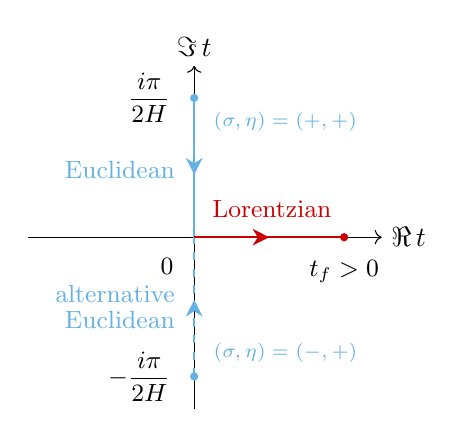
\begin{tikzpicture}[
    scale=0.68,
    baseline=(current bounding box.center),
    mid arrow/.style={
        postaction={
            decorate,
            decoration={
                markings,
                mark=at position 0.5 with
                {\arrow{Stealth[length=6pt,width=6pt]}}
            }
        }
    }
]

\pgfdeclareradialshading{inflationellipse}{\pgfpoint{0cm}{0cm}}{
  color(0cm)=(red4!80);
  color(0.6cm)=(orange!40);
  color(0.9cm)=(yellow!10)
}

% Axes
\draw[->] (-3.1,0) -- (3.5,0)
node[right] {$\Re\,t$};

\draw[->] (0,-3.2) -- (0,3.2)
node[above] {$\Im\,t$};

% Upper Euclidean contour: (sigma,eta)=(+,+)
\draw[
    thick,
    cornflowerblue,
    postaction={
        decorate,
        decoration={
            markings,
            mark=at position 0.55 with
            {\arrow{Stealth[length=6pt,width=6pt]}}
        }
    }
]
(0,2.6) -- (0,0);

% Lower alternative Euclidean contour: (sigma,eta)=(-,-)
\draw[
    thick,
    cornflowerblue,
    dashed,
    postaction={
        decorate,
        decoration={
            markings,
            mark=at position 0.55 with
            {\arrow{Stealth[length=6pt,width=6pt]}}
        }
    }
]
(0,-2.6) -- (0,0);

% Common Lorentzian segment
\draw[
    thick,
    red4,
    mid arrow
]
(0,0) -- (2.8,0);

% End points
\fill[cornflowerblue] (0,2.6) circle (2.2pt);
\fill[cornflowerblue] (0,-2.6) circle (2.2pt);
\fill[red4] (2.8,0) circle (2.2pt);

% Endpoint labels
\node[left=5pt] at (0,2.6)
{\small $\displaystyle \frac{i\pi}{2H}$};

\node[left=5pt] at (0,-2.6)
{\small $\displaystyle -\frac{i\pi}{2H}$};

\node[below=5pt] at (2.8,0)
{\small $t_f>0$};

% Origin
\node[below left=4pt] at (0,0)
{\small $0$};

% Region labels
\node[cornflowerblue,left] at (-0.18,1.25)
{\small Euclidean};

\node[cornflowerblue,left,align=right] at (-0.18,-1.30)
{\small alternative\\[-1mm]\small Euclidean};

\node[red4,above] at (1.45,0.18)
{\small Lorentzian};

% Saddle labels
\node[cornflowerblue,right] at (0.18,2.15)
{\scriptsize $(\sigma,\eta)=(+,+)$};

\node[cornflowerblue,right] at (0.18,-2.15)
{\scriptsize $(\sigma,\eta)=(-,+)$};

\end{tikzpicture}

\end{subfigure}
\hfill
% ============================================================
% RIGHT PANEL
% ============================================================
\begin{subfigure}[c]{0.54\textwidth}
\centering

\raisebox{-1.1\height}{
\resizebox{0.6\linewidth}{!}{
\begin{tikzpicture}[xscale=0.35,yscale=0.4]

% Euclidean hemisphere
\path[fill=cyan!10, opacity=0.3]
    (2,2)
    arc[  start angle=90,  end angle=270,  x radius=2,  y radius=2 ]
    -- (2,-2) -- cycle;

\draw[thick,cornflowerblue]
    (2,2)
    arc[ start angle=90, end angle=270,  x radius=2,  y radius=2 ];

% no-boundary label
\draw[ thick, navyblue, decorate, decoration={
        text along path,
        text={|\tiny|no-boundary},
        text align=center,
        text color=navyblue,
        reverse path,
        raise=3.5pt,
        text format delimiters={|}{|}
    }
]
(2,2)
arc[start angle=90, end angle=270, x radius=2, y radius=2];

% Lorentzian region
\path[fill=red,opacity=0.08]
 (1.4,0)
 arc[ start angle=180, end angle=-90, x radius=0.6, y radius=2]
 .. controls (3.5,-2) .. (6.1,-3)
 arc[ start angle=-90, end angle=90, x radius=1, y radius=3
 ]
 .. controls (3.5,2) .. (2,2)
 arc[ start angle=90,  end angle=180,  x radius=0.6,  y radius=2 ]
 -- cycle;

% Matching surface
\shade[
    shading=inflationellipse,
    opacity=0.6
]
(2,0) ellipse (0.6 and 2);

% Lorentzian boundaries
\draw[thick,red4]
(6.1,0) ellipse (1 and 3);

\draw[thick,red4,dotted]
(2,0) ellipse (0.6 and 2);

\draw[thick,red4]
(2,2)
.. controls (3.5,2) ..
(6,3);

\draw[thick,red4]
(2,-2)
.. controls (3.5,-2) ..
(6,-3);

% Inflation label
\draw[thick, red4, decorate, decoration={
        text along path,
        text={|\scriptsize|Inflation},
        text align=center,
        text color=red4,
        reverse path,
        raise=0pt,
        text format delimiters={|}{|}
    }
]
(2.2,3)
arc[
    start angle=95,
    end angle=-90,
    x radius=1,
    y radius=3
];

% Lorentzian evolution label
\draw[ thick, red4, decorate, decoration={
        text along path,
        text={|\tiny|Lorentzian evolution},
        text align=center,
        text color=red4,
        reverse path,
        raise=0pt,
        text format delimiters={|}{|}
    }
]
(6.8,3)
arc[ start angle=90, end angle=-90,  x radius=1,  y radius=3
];

% Horizontal Euclidean time line
\draw[->, line width=0.9pt, opacity=0.2]
(0,0) -- (2,0);

\node[above] at (1.1,0)
{\scriptsize\color{gray}$\tau$};

% Horizontal Lorentzian time line
\draw[
    ->,
    line width=0.9pt,
    opacity=0.2
]
(2.2,0) -- (6.6,0);

\node[above] at (6,0)
{\scriptsize\color{gray}$t$};

\end{tikzpicture}
}}
\end{subfigure}

\caption{No-boundary saddle and its analytic continuation.
\emph{Left:} Representative contours in the complex $t$ plane for the two orientations of the Wick rotation that lead to the same expanding Lorentzian geometry at $t_f>0$. The solid and dashed Euclidean segments correspond to $(\sigma,\eta)=(+,+)$ and $(-,+)$, respectively, and run from $t=\pm i\pi/(2H)$ to the turning surface at $t=0$. Both contours then continue along the positive real axis, describing Lorentzian evolution.
\emph{Right:} Geometric interpretation of the analytic continuation. The Euclidean no-boundary hemisphere is smoothly joined at its equator to an expanding Lorentzian de Sitter spacetime.}
\label{fig:no-boundary-contour}

\end{figure}
Consequently, for a fixed Wick-rotation orientation one obtains two complex-conjugate Euclidean saddles,
\begin{equation}
    \mathcal{S}_E^{(\eta)}
    =-\frac{4\pi^2}{\kappa H^2}
    \left[
        1-\eta\,i\left((bH)^2-1\right)^{3/2}
    \right]\,,
    \qquad \eta=\pm1\,.
\end{equation}
There is a second, independent sign choice associated with the orientation of the Wick rotation. This becomes particularly manifest when the instantons are regarded as saddles of the Lorentzian path integral. We define
$\sigma=+1$ for $t=-i\tau$ and
$\sigma=-1$ for $t=+i\tau$. Correspondingly,
$i\mathcal{S}_L=-\mathcal{S}_E$ for $\sigma=+1$, whereas
$i\mathcal{S}_L=+\mathcal{S}_E$ for $\sigma=-1$. The Lorentzian saddle exponents can therefore be written compactly as
\begin{equation}\label{eq:Complexinstantons}
    i\mathcal{S}_L^{(\sigma,\eta)}
    =\sigma\,\frac{4\pi^2}{\kappa H^2}
    \left[
        1-\eta\,i\big((bH)^2-1\big)^{3/2}
    \right]\,,
    \qquad \sigma,\eta=\pm1\,.
\end{equation}
The origin of the four semiclassical saddle contributions in
Eq.~\eqref{eq:Complexinstantons} is thus transparent.  The parameter
$\eta$ labels the two branches compatible with the same final scale factor, while $\sigma$ specifies the orientation of the Wick rotation.
At this stage, it is relevant to note that we didn't say anything about the contour in the complex plane. A convenient representative of contour for the $(\sigma =1, \eta =1)$ instanton starts at the South Pole $t=i\pi/(2H)$, runs along the imaginary axis to the turning surface $t=0$, and then continues along the real axis up to $t=-i\tau_f>0$. Geometrically, this describes a Euclidean half-sphere smoothly joined at its equator to an expanding Lorentzian de Sitter spacetime. The ($\sigma=-1,\eta=1$) is obtained by reflecting the Euclidean part of the contour across the imaginary $t$ axis. \PG{I have the problem that if $\eta>0$ and we choose $\tau_f$ purely imaginary then $\Im(\tau_f)>0$ so $t_f = i \tau_f <0$ for the Tunneling proposal. Do we agree on that ?} \IG{I think yes. Does this make sense?}\PG{This is not a big deal because the scale factor is even but it then means that the Tunelling instanton runs backward in time.} The right panel of Fig.~\ref{fig:no-boundary-contour} displays the corresponding geometric interpretation: a Euclidean half-sphere smoothly joined at its equator to an expanding Lorentzian de Sitter spacetime. The piecewise-linear contours shown in Fig.~\ref{fig:no-boundary-contour} should only be regarded as convenient
representatives. For fixed endpoints and a fixed analytic branch of the saddle, the on-shell action is invariant under continuous deformations of the contour.
 
The result~\eqref{eq:Complexinstantons} is the exact de Sitter limit of the slow-roll solution. For a
slowly evolving scalar field, deviations from this limit can be organized perturbatively in terms of the usual potential slow-roll parameters,
\begin{equation}
    \epsilon_V = \frac{1}{2 \kappa} \left(\frac{V_{\phi}}{V}\right)^2\ll1\,,\qquad \eta_V = \frac{1}{ \kappa} \frac{V_{\phi \phi}}{V}\,, \qquad |\eta_V|\ll 1\,.
\label{eq:slow_roll}
\end{equation}
Such corrections deform both the Euclidean instanton and its Lorentzian continuation away from exact de Sitter space and can be incorporated systematically within a slow-roll expansion (see~\cite{Maldacena:2024uhs,Janssen_2021} and references therein).

It is also useful to clarify a point of terminology. What are usually referred to as the Hartle-Hawking and Vilenkin proposals correspond to a choice of boundary conditions for the WKB wavefunction of the universe obeying the Wheeler-DeWitt equation. These boundary conditions determine which linear combination of the no-boundary saddles
discussed above contributes to the wave function of the universe.

\PG{I have the issue that when solving the Wheeler-DeWitt equation in minisuperspace in the extra slow roll regime, the $\phi$ dependence disappears and thus the overall factor $\exp\left(\pm\frac{4 \pi^2}{\kappa \tilde{V}}\right) = \exp\left(\pm\frac{4 \pi^2}{\kappa H^2}\right)$ seems to be a constant.} \IG{If you assume that $\tilde{V} = H^2$, then yes the overall factor is a constant.}\PG{Maybe, look at the appendix, you will understand my problem. Essentially, solving the Wheeler-DeWitt equation in the extra slow-roll limit does not tell anything about the prefactor. It seems to be that only the Lorentzian path-integral can allow you to define properly the boundary conditions. Or, you have to re-establish the $\phi$-dependence somehow...}
In the classically forbidden region $aH<1$, the Hartle–Hawking prescription selects the growing WKB branch. Matching this solution across the turning point at $aH=1$ produces, in the classically allowed region, a real superposition of expanding and contracting WKB branches. In terms of the saddle labels introduced above, this corresponds to the
two complex-conjugate saddles with $\sigma=+1$ and $\eta=\pm1$. Their sum gives
\begin{equation}
    \Psi_{HH} \propto \exp\left(\frac{4\pi^2}{\kappa H^2}\right)\cos\left[{\color{blue} \frac{4\pi^2}{\kappa H^2}}\left((bH)^2-1\right)^{3/2}-\frac{\pi}{4}\right]\,.
\end{equation}
 The characteristic enhancement $\exp(4\pi^2/\kappa H^2)$ originates from the real part of the Euclidean no-boundary action, while the two complex-conjugate saddles combine into an oscillatory WKB wave function in the Lorentzian region. The additional phase shift $-\pi/4$ arises from the standard WKB connection formula at the turning point $aH=1$, or equivalently from the associated Maslov--Morse index; see, for instance, Ref.~\cite{PhysRevD.37.888}.

By contrast, Vilenkin's tunnelling prescription is imposed in the classically allowed region and selects the outgoing branch so $\sigma \eta =-1$. In fact, the Tunneling prescription only picks out the instanton with $(\sigma =-1,\eta=1)$, yielding
\begin{equation}
    \Psi_T \propto \exp\left(-\frac{4\pi^2}{\kappa H^2}\left[1+i\left((bH)^2-1\right)^{3/2}\right]\right)\,
\end{equation}
{\color{blue} Thus, although the Hartle--Hawking and tunnelling wave functions are constructed from the same set of complex no-boundary saddles, they differ in the prescription used to select and combine them.}

\PG{Say something more precise concerning the Lorentzian path-integral formulation}
In a Lorentzian path-integral formulation, the wave function may be written schematically as
\begin{equation*}
    \Psi
    \propto
    \int_{\mathcal{C}_N}{\rm d}N
    \int_{B_i}^{B_f}
    \mathcal{D}a\,\mathcal{D}\phi\,
    e^{i\mathcal{S}_L[a,\phi,N]}\,.
\end{equation*}
From this perspective, which complex saddles actually contribute is determined not only by the boundary conditions, but also by the choice of lapse contour $\mathcal{C}_N$ and by the boundary terms included in the action. Different contour prescriptions can therefore select different combinations of the available saddle points. For further discussions, see~\cite{PhysRevD.39.2206,Lehners:2023yrj,Vilenkin_2018,Feldbrugge:2017kzv,
Feldbrugge:2017fcc,DiazDorronsoro:2017hti}.

\subsection{Analytic wineglass wormhole backgrounds}

We now turn to the wineglass background. Starting from the Einstein--scalar system introduced above, we supplement the matter sector by primordial gauge fields,\footnote{More generally, the same role can be played by primordial axionic fields~\cite{Betzios:2024oli}.} which play an essential role in supporting the Euclidean wormhole geometries of interest. The Euclidean action is
\begin{equation}\label{background}
\mathcal{S}_E = \int {\rm d}^4x \sqrt{g_E} \left(-\frac{\mathcal{R}}{2\kappa} + \frac12 (\partial_\mu\phi)^2 +V(\phi) + \mathcal{L}_{\rm rad}^E \right)+\mathcal{S}_{\rm GHY}\,.
\end{equation}
We restrict again to closed FLRW geometries. The Euclidean and Lorentzian line elements are
\begin{equation}\label{eq:analyticcontinuation}
{\rm d}s_E^2={\rm d}\tau^2+a^2(\tau){\rm d}\Omega_3^2\,,
\qquad \longleftrightarrow \qquad
{\rm d}s_L^2=-{\rm d}t^2+a^2(t){\rm d}\Omega_3^2\,,
\end{equation}
and are related by analytic continuation in the complexified time plane $t=\pm i\tau$. The class of potentials supporting half-wormhole, or ``wineglass'', geometries that interpolate between an asymptotically EAdS Euclidean region and an asymptotically de Sitter Lorentzian region was discussed in~\cite{Betzios:2024oli}. A representative potential is shown in Fig.~\ref{fig:potentialhistory}.
\begin{figure}[htb]
\centering
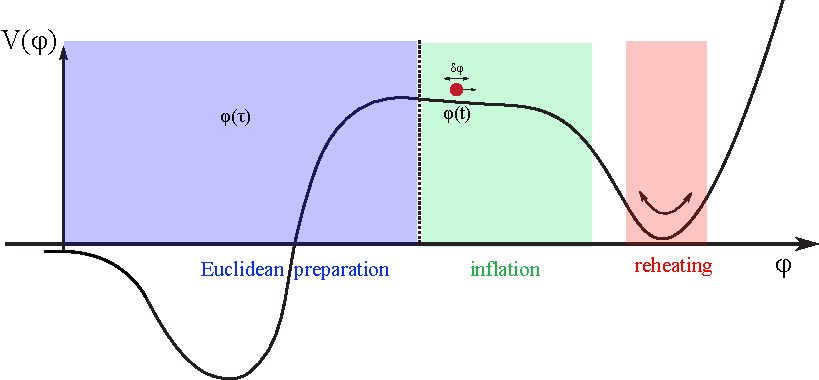
\includegraphics[width=0.8\linewidth]{Figures_paper_2/PotentialHistory.pdf}
\caption{Representative scalar potential supporting half-wormhole wineglass solutions.}
\label{fig:potentialhistory}
\end{figure}

For the explicit realization based on three $U(1)$ gauge fields, the phase space of homogeneous and isotropic Euclidean solutions was analyzed in detail in~\cite{Betzios:2026rbv}. This construction provides a framework for comparing different Euclidean preparations of the universe and their relative semiclassical weights. Here we restrict attention to the branch that gives rise, after analytic continuation, to the inflationary background relevant for the perturbation analysis below.

We consider the homogeneous and isotropic ansatz\footnote{In our previous work~\cite{Betzios:2026rbv}, the gauge potential was denoted by $H(\tau)$. Here we use $W(\tau)$ in order to avoid confusion with the Hubble scale.}
\begin{equation}
    \rm{d}s^2 = \rm{d}\tau^2 + a^2(\tau) \rm{d}\Omega_3^2\,, \quad \phi = \phi(\tau)\,, \quad A^{(I)}(\tau) = \omega^{(I)} W(\tau)\,,
\end{equation}
where $\omega^{(I)}$ are the Maurer--Cartan one-forms on $S^3$, satisfying $ {\rm d}\omega^{(I)}=\frac{1}{2}\epsilon^{I}{}_{JK} \omega^{(J)}\wedge\omega^{(K)}\,.$
The Euclidean equations of motion are
\begin{align}
\tilde{\phi}''+3\frac{a'\tilde{\phi}'}{a}-\frac{{\rm d}\tilde{V}(\phi)}{{\rm d} \tilde{\phi}} &= 0\,, \nonumber
\\
\frac{2a''}{a}+\frac{a'^2}{a^2}-\frac{1}{a^2}  + 3 \left(\tilde{V}(\phi)+\frac{\tilde{\phi}'^2}{2} \right) +  \frac{\tilde{\rho}^E_{\rm rad}}{a^4} & =0  \,, \nonumber
\\
\frac{a'^2}{a^2} -\frac{1}{a^2}  + \left(\tilde{V}(\phi)-\frac{\tilde{\phi}'^2}{2} \right) - \frac{\tilde{\rho}^E_{\rm rad}}{a^4} & =0 \,, \nonumber
\\
W''+\frac{a'}{a}W'-\frac{4W}{a^2} &=0
\,.
\label{eq:eoms_Eucl}
\end{align}
The gauge-field equation implies that the Euclidean radiation density is conserved. More explicitly,
\begin{equation}
\tilde{\rho}^E_{\rm rad} = 2\kappa a^4 \left[ \left(\frac{W'}{a} \right)^2 - \frac{4W^2}{a^4} \right] = \rm const <0\,.
\label{eq:rhoE_rad_W}
\end{equation}
Introducing the conformal coordinate  $u = \int_{{\color{blue}0}}^{\tau} \rm{d}\tau'/a(\tau')$, the $\mathbb{Z}_2$-symmetric wineglass solution is even around the turning surface at $u=0$, with $W(u)=W_0\cosh(2u)$. Therefore $W'(0)=0$, while $W(0)=W_0\neq0$. Evaluating~\eqref{eq:rhoE_rad_W} at the turning surface gives
\begin{equation}
\tilde{\rho}^E_{\rm rad} = -8\kappa W_0^2<0 \,.
\end{equation}
Thus, the Euclidean radiation density is negative for the $\mathbb{Z}_2$-symmetric wineglass branch.

The precise form of the scalar potential and the corresponding family of solutions are discussed in detail in~\cite{Betzios:2026rbv}. Here we focus on the analytic solution obtained when the scalar source at the asymptotic EAdS boundary is switched off. The Euclidean half-wineglass consists of two regions. Region~{\bf I} contains the asymptotic EAdS boundary, while Region~{\bf II} connects it to the turning surface at $\tau=0$. The scale factor is
\begin{equation}
 a_{H-WG}^2(\tau) = 
    \begin{cases}
   \displaystyle   \frac{1}{4 H_{\rm I}^2\cosh(\bar{\tau}^{\textbf{I}})}\left(\sqrt{A_{\rm I}}\cosh{(\bar{\tau}^{\textbf{I}})}-\frac{1}{\sqrt{A_{I}}}\right)^2\,, \quad\,\,\,\,\, \tau \leq -\frac{\pi}{2H_{\rm II}}\,, \quad (\textbf{I}) &  
\\[0.3cm]
   \displaystyle     \frac{1}{4 H_{\rm II}^2} \left(\cos{(2H_{\rm II}\tau)}+ c_{\rm II}\right)\,,  \hspace{1.8cm}  -\frac{\pi}{2H_{\rm II}} \leq \tau \leq 0\,.  \hspace{1.2cm} (\textbf{II}) &
\end{cases}
\label{eq:background_ans_simple}
\end{equation}
Here we have introduced the dimensionless variables $\bar{\tau}^{\textbf{I}}=2H_{\rm I}(\tau-\tau_{\rm min})$
and $\bar{\tau}^{\textbf{II}}=2H_{\rm II}\tau$, with the matching point between the two regions located at $\tau_{\rm min} = -\pi/(2H_{II})$. The parameters satisfy
\begin{equation}
    A_I = \frac{1+\sqrt{5}}{2}\,, \quad
    c_{\rm II} = -16H_{\rm II}^2\tilde{\rho}^E_{\rm rad}-1\,, \quad
    H_I^2 = H^2_{II}\frac{\sqrt{5}-2}{-16\tilde{\rho}^E_{\rm rad}H_{\rm II}^2-2}\,.
\end{equation}
% \begin{equation}
% \begin{aligned}
%     A_I &= \frac{1+\sqrt{5}}{2}\,,\\
%     c_{\rm II} &= -16H_{\rm II}^2\tilde{\rho}^E_{\rm rad}-1\,,\\
%     H_I^2 &= H^2_{II}\frac{\sqrt{5}-2}{-16\tilde{\rho}^E_{\rm rad}H_{\rm II}^2-2}\,.
% \end{aligned}
% \end{equation}

There are two distinct ways of extending the Euclidean half-saddle beyond the turning surface at $\tau=0$. One possibility is to reflect the solution across $\tau=0$, producing the complete Euclidean wineglass wormhole $a_{\rm WG}$. Alternatively, for cosmological applications, the Euclidean half-saddle can be analytically continued through the turning surface into a Lorentzian spacetime. These two constructions therefore coincide throughout the Euclidean branch up to $\tau=0$, but describe physically different continuations beyond it. This distinction is illustrated in Fig.~\ref{fig:wormholes}.

We denote the analytically continued configuration by
\begin{equation}
\left( a_{\rm H\text{-}WG},
\phi_{\rm H\text{-}WG},
\tilde{\rho}_{\rm rad}^{L} \right), \qquad \tilde{\rho}_{\rm rad}^{L} = -\tilde{\rho}_{\rm rad}^{E}>0\,.
\end{equation}
The sign reversal of the effective radiation density follows from the analytic continuation of the gauge sector.\footnote{
The Lorentzian radiation density is
\begin{equation}
    \tilde{\rho}_{\rm rad}^{L}:= 2\kappa a^4 \left[
  \left(\frac{\dot{W}}{a}\right)^2  +\frac{4W^2}{a^4}
    \right] = {\rm const}>0\,.
\end{equation}
The gauge potential is $\mathcal{C}^1$ along the complex contour. In particular, its velocity vanishes at the turning surface, so that
$\tilde{\rho}_{\rm rad}^{L}
=-\tilde{\rho}_{\rm rad}^{E}$.
}

The Lorentzian evolution is governed by
\begin{align}
\ddot{\tilde{\phi}}+3\frac{\dot a\dot{\tilde{\phi}}}{a} + \frac{{\rm d}\tilde{V}(\phi)}{{\rm d} \tilde{\phi}} &= 0\,, \nonumber
\\
\frac{2 \ddot a}{a} + \frac{\dot a^2}{a^2} + \frac{1}{a^2}  - 3 \left(\tilde{V}(\phi) - \frac{\dot{\tilde{\phi}}^2}{2} \right) +  \frac{\tilde{\rho}^L_{\rm rad}}{a^4} & =0  \,, \nonumber
\\ 
 \frac{\dot a^2}{a^2} +\frac{1}{a^2}  - \left(\tilde{V}(\phi) + \frac{\dot{\tilde{\phi}}2}{2} \right) - \frac{\tilde{\rho}^L_{\rm rad}}{a^4} & =0 \,,
\nonumber
\\
\ddot W+\frac{\dot a}{a}\dot W+\frac{4W}{a^2} &=0\,.
\label{eq:eoms_Lor}
\end{align}
\begin{figure}[t!]
\centering

\begin{subfigure}{0.48\textwidth}
\centering
\resizebox{!}{2.8cm}{
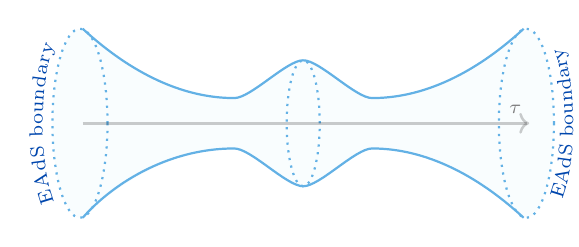
\begin{tikzpicture}[xscale=0.35, yscale=0.4]
\hspace{0.3cm}

\path[fill=cyan!10, opacity=0.25]
  (-7.1,0)
arc[start angle=180,end angle=270,x radius=1,y radius=3] 
  .. controls (-5.,-2.2) and (-3.,-0.8) .. (-0.5,-0.8)
  .. controls (0.1,-0.8) and (1.4,-2) .. (2.,-2)     
arc[start angle=-90,end angle=-270,x radius=0.6,y radius=2]
  .. controls (1.4,2) and (0.1,0.8) .. (-0.5,0.8)
  .. controls (-3.,0.8) and (-5.,2.2) .. (-6.1,3)
arc[start angle=90,end angle=180,x radius=1,y radius=3]
  -- cycle;

\path[fill=cyan!10, opacity=0.25]
  (10.1,-3)
  .. controls (9.,-2.2) and (7.,-0.8) .. (4.5,-0.8)
  .. controls (3.9,-0.8) and (2.6,-2.) .. (2,-2)
arc[start angle=-90,end angle=-270,x radius=0.6,y radius=2]
  .. controls (2.6,2.) and (3.9,0.8) .. (4.5,0.8)
  .. controls (7.,0.8) and (9.,2.2) .. (10.1,3)
arc[start angle=90,end angle=-90,x radius=1,y radius=3]
  -- cycle;

\draw[thick, cornflowerblue, dotted] (-6.1,0) ellipse (1 and 3);
\draw[thick,  cornflowerblue, dotted] (2,0) ellipse (0.6 and 2);
\draw[thick,  cornflowerblue, dotted] (10.1,0) ellipse (1 and 3);


\draw[thick, navyblue, decorate,
      decoration={
          text along path,
          text={|\scriptsize|EAdS boundary},
          text align=center,
          text color=navyblue,
          reverse path,
          raise=3.5pt,
          text format delimiters={|}{|}
      }
]
(-6.1,3) arc[start angle=90,end angle=270,x radius=1,y radius=3];


\draw[thick, navyblue, decorate,
      decoration={
          text along path,
          text={|\scriptsize|EAdS boundary},
          text align=center,
          text color=navyblue,
          reverse path,
          raise=0.pt,
          text format delimiters={|}{|}
      }
]
(10.8,3) arc[start angle=90,end angle=-90,x radius=1,y radius=3];


\draw[thick, cornflowerblue]
  (-6,3) .. controls (-5.,2.2) and (-3,0.8) .. (-0.5,0.8)
        .. controls (.1,0.8) and (1.4,2.) .. (2,2);

\draw[thick, cornflowerblue]
  (10,3) .. controls (9,2.2) and (7.,0.8) .. (4.5,0.8)
        .. controls (3.9,0.8) and (2.6,2.) .. (2,2);

\draw[thick, cornflowerblue]
  (-6,-3) .. controls (-5.,-2) and (-3,-0.8) .. (-0.5,-0.8)
         .. controls (0.1,-0.8) and (1.4,-2.) ..(2,-2);

\draw[thick, cornflowerblue]
  (10,-3) .. controls (9.,-2.2) and (7.,-0.8) .. (4.5,-0.8)
        .. controls (3.9,-0.8) and (2.6,-2.) .. (2,-2);

\draw[->,  line width=0.9pt,  opacity=0.2] (-6,0) -- (10.2,0);
\node[above] at (9.7,0.) {\scriptsize\color{gray}$\tau$};

\end{tikzpicture}
}
\end{subfigure}
\hfill
\begin{subfigure}{0.4\textwidth}
\centering
\resizebox{!}{2.8cm}{
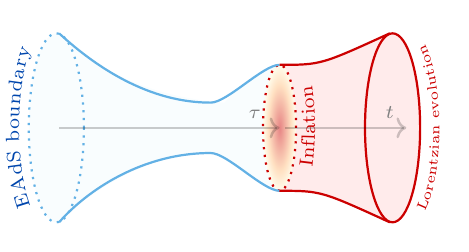
\begin{tikzpicture}[xscale=0.35, yscale=0.4]

\path[fill=cyan!10, opacity=0.25]
  (-7.1,0)
  arc[start angle=180,end angle=270,x radius=1,y radius=3] 
  .. controls (-5,-2.2) and (-3,-0.8) .. (-0.5,-0.8)
  .. controls (0.1,-0.8) and (1.4,-2) .. (2,-2)     
  arc[start angle=-90,end angle=-270,x radius=0.6,y radius=2]
  .. controls (1.4,1.95) and (0.6,1.4) .. (0,0.8)
  .. controls (-3,1) and (-4.8,2) .. (-6.1,3)
  arc[start angle=90,end angle=180,x radius=1,y radius=3]
  -- cycle;

\path[fill=red, opacity=0.08]
  (1.4,0)
  arc[start angle=180,end angle=-90,x radius=0.6,y radius=2] 
  .. controls (3.5,-2) .. (6.1,-3)                    
  arc[start angle=-90,end angle=90,x radius=1,y radius=3]  
  .. controls (3.5,2) .. (2,2)                        
  arc[start angle=90,end angle=180,x radius=0.6,y radius=2]  
  -- cycle;

\pgfdeclareradialshading{inflationellipse}{\pgfpoint{0cm}{0cm}}{
  color(0cm)=(red4!80);
  color(0.6cm)=(orange!40);
  color(0.9cm)=(yellow!10)
}

\shade[shading=inflationellipse, opacity=0.6] (2,0) ellipse (0.6 and 2);


\draw[thick, navyblue, decorate,
      decoration={
          text along path,
          text={|\scriptsize|EAdS boundary},
          text align=center,
          text color=navyblue,
          reverse path,
          raise=3.5pt,
          text format delimiters={|}{|}
      }
]
(-6.1,3) arc[start angle=90,end angle=270,x radius=1,y radius=3];

\draw[thick, red4, decorate,
      decoration={
          text along path,
          text={|\scriptsize|Inflation},
          text align=center,
          text color=red4,
          reverse path,
          raise=0.pt,
          text format delimiters={|}{|}
      }
]
(2.2,3) arc[start angle=95,end angle=-90,x radius=1,y radius=3];



\draw[thick, red4, decorate,
      decoration={
          text along path,
          text={|\tiny|Lorentzian evolution},
          text align=center,
          text color=red4,
          reverse path,
          raise=0.pt,
          text format delimiters={|}{|}
      }
]
(6.8,3) arc[start angle=90,end angle=-90,x radius=1,y radius=3];



\draw[thick, cornflowerblue, dotted] (-6.1,0) ellipse (1 and 3);
\draw[thick, red4] (6.1,0) ellipse (1 and 3);
\draw[thick, red4, dotted] (2,0) ellipse (0.6 and 2);

\draw[thick, cornflowerblue]
  (-6,3) .. controls (-5.,2.2) and (-3,0.8) .. (-0.5,0.8)
        .. controls (.1,0.8) and (1.4,2.) .. (2,2);

\draw[thick, red4] (2,2) .. controls (3.5,2) .. (6,3);

\draw[thick, cornflowerblue]
  (-6,-3) .. controls (-5.,-2) and (-3,-0.8) .. (-0.5,-0.8)
         .. controls (0.1,-0.8) and (1.4,-2.) .. (2,-2);

\draw[thick, red4] (2,-2) .. controls (3.5,-2) .. (6,-3);

\draw[->,  line width=0.9pt,  opacity=0.2] (-6,0) -- (2,0);
\node[above] at (1.1,0.) {\scriptsize\color{gray}$\tau$};

\draw[->,  line width=0.9pt,  opacity=0.2] (2.2,0) -- (6.6,0);
\node[above] at (6.,0.) {\scriptsize\color{gray}$t$};

\end{tikzpicture}
}
\end{subfigure}

\caption{Schematic illustration of the wineglass wormhole proposal for the birth of the Universe. 
\emph{Left:} The Euclidean wineglass wormhole geometry connecting two asymptotic EAdS boundaries. 
\emph{Right:} The half-wineglass wormhole evolves into a Lorentzian quasi-$dS_4$ spacetime describing an expanding universe after the junction point at $t=\tau=0$.}
\label{fig:wormholes}
\end{figure}
The analytic continuation changes the character of the turning surface. Along the Euclidean direction, $\tau=0$ is a local maximum of $a(\tau)$, whereas along the Lorentzian direction it becomes a local minimum of $a(t)$. Similarly, the sign of the acceleration induced by the scalar potential is reversed across the continuation.

The complete Euclidean wineglass therefore remains entirely within the Euclidean preparation region of the potential, shown in blue in Fig.~\ref{fig:potentialhistory}. In the half-wineglass construction, by contrast, the scalar crosses the junction and subsequently evolves through the inflationary region, shown in red, before eventually approaching the reheating region shown in green \IG{[change colors in the plot]}. The Euclidean half-wormhole therefore prepares the initial conditions for the subsequent Lorentzian cosmology.


To obtain an analytic expression for the Lorentzian background, we assume that the scalar evolves in the slow-roll regime introduced in eq.~\eqref{eq:slow_roll}. At leading order in slow-roll, its kinetic energy can be neglected and the potential can be treated as approximately constant,
\begin{equation}
    \tilde{V}(\phi) = \tilde{V}\big|_{\tau=0}
    \equiv \tilde{V}_0  =  H^2\,.
\end{equation}
The Lorentzian Friedmann equation can then be solved analytically, yielding
\begin{equation}\label{eq:Lorentzian_wineglass}
    a^2_{\rm H\text{-}WG}(t) = \frac{2+\cosh(2Ht)}{4H^2}+\mathcal{O}(H^{-2}\epsilon_V,H^{-2}\eta_V)\,, \quad H^2 = \frac{3}{16 \tilde{\rho}^L_{\rm rad}}\,.
\end{equation}
In this solution, the asymptotic de Sitter scale $H$ is fixed by the conserved Lorentzian gauge-field energy density. The background may therefore be parametrized by the pair $(\tilde{\rho}_{\rm rad}^{L},H_{\rm II})$, or equivalently by $(H,H_{\rm II})$. At the maching surface
\begin{equation}
     a_{\rm H\text{-}WG}^2(0) = \frac{3}{4H^2}\,,
    \qquad
    \dot a_{\rm H\text{-}WG}(0)=0\,,
\end{equation}
confirming explicitly that the Lorentzian evolution begins at a nonvanishing minimum radius. At late Lorentzian times,
\begin{equation}
    a_{\rm H\text{-}WG}(t) =
    \frac{e^{Ht}}{2\sqrt{2}\,H} \left[ 1+\mathcal{O}(e^{-2Ht}) \right]\,.
\end{equation}
The half-wineglass background therefore asymptotes exponentially to de Sitter space. Comparing with eq.~\eqref{eq:ansatzs_scalefactor}, its asymptotic normalization corresponds to $\alpha_{\rm WG}= 1/\sqrt{2}$ in contrast to $\alpha_{\rm NB}=1$ for the exact no-boundary de Sitter solution.


In what follows, we neglect slow-roll corrections to the analytic background. They can be incorporated systematically as perturbative corrections to both the scale factor and the scalar profile,
$\phi=\phi_\star+\delta\phi$; see, for example, Ref.~\cite{Maldacena:2004rf}.\footnote{
For the wineglass solutions of interest, an exactly flat potential with
$\epsilon_V=\eta_V=0$ is not strictly admissible, since a nonvanishing scalar evolution is required to interpolate between the Euclidean preparation region and the Lorentzian inflationary regime. The exact de Sitter result should therefore be understood as the leading term in a slow-roll expansion.}
\begin{equation}
 a_{\rm H\text{-}WG}^2 = 
    \begin{cases}
   \displaystyle   \frac{1}{4 H_{\rm I}^2\cosh(\bar{\tau}^{\textbf{I}})}\left(\sqrt{A_{\rm I}}\cosh{(\bar{\tau}^{\textbf{I}})}-\frac{1}{\sqrt{A_{I}}}\right)^2\,, \quad\,\,\,\,\, \tau \leq -\frac{\pi}{2H_{\rm II}}\,,  \hspace{0.7cm}   (\textbf{Eucl.  I})&
\\[0.3cm]
   \displaystyle     \frac{1}{4 H_{\rm II}^2} \left(\cos{(\bar{\tau}^{\textbf{II}})}+ c_{\rm II}\right)\,,  \hspace{2.2cm}  -\frac{\pi}{2H_{\rm II}} \leq \tau \leq 0\,,  \hspace{1.65cm}  (\textbf{Eucl. II}) &
\\[0.3cm]
  \displaystyle     \frac{2+\cosh(\bar{t})}{4H^2} \,, \hspace{5.5cm}  \bar{t} = 2Ht \geq0\,. \hspace{0.6cm} (\textbf{Lorentzian})&  
\end{cases}
\label{eq:background_ans_simple_2}
\end{equation}
% \PG{I would rather prefer eliminating $c_{\rm II}$ everywhere...}
% \begin{equation}
% \begin{aligned}
% H_{\rm II}^2 &= H_{\rm I}^2\, \frac{c_{\rm II}-1}{\sqrt{5}-2}\,, & H^2 &= \frac{3H_{\rm II}^2}{c_{\rm II}+1}\,,
% \\[0.2cm]
% \tilde{\rho}_{\rm rad}^{E} &= -\frac{c_{\rm II}+1}{16H_{\rm II}^2}\,, &
% \tilde{\rho}_{\rm rad}^{L} &= \frac{3}{16H^2}\,.
% \end{aligned}
% \end{equation}




\section{Cosmological perturbations}\label{sec:cosmological_perturbations}
In what follows, we study a probe massless scalar field propagating on two different semiclassical backgrounds: the standard no-boundary geometry and the “wineglass” wormhole geometry. Since the dynamics of the background is treated independently of the probe field, our analysis amounts to quantum field theory on a fixed classical spacetime. In both cases, however, the relevant saddle discussed in section~\ref{sec:Background} consists of a Euclidean region smoothly connected to a Lorentzian cosmological evolution. It is well known that in quantum field theory, in order to render the correlation functions well defined a certain $i\epsilon$ prescription should be incorporated. In the Hartle–Hawking framework~\cite{Hartle:1983ai}~\cite{Halliwell:1984eu}, canonical quantum cosmology gives this Euclidean continuation a geometrical interpretation: the Euclidean portion of the saddle prepares the quantum state from which the subsequent Lorentzian universe evolves. The precise form of this Euclidean region depends on the matter content of the theory and on the corresponding semiclassical Einstein equations. The No-boundary and wineglass proposals therefore differ already at zeroth order in perturbation theory: their minisuperspace equations select distinct Euclidean geometries and impose different conditions at the initial end of the contour. These different state-preparation geometries lead to different mode functions after analytic continuation, even when the two backgrounds approach the same Lorentzian de Sitter geometry at late times. Studying how the Euclidean part of the saddle affects late-time cosmological correlators thus provides a controlled way of probing the semi-classical imprint of quantum-gravitational initial conditions. More precisely, it allows us to isolate how different geometrical prescriptions for preparing the cosmological state modify observables such as the late-time power spectrum.


This section is organized as follows. The first part gives general analytical results independent of the background geometry assuming only that the late-time Lorentzian universe asymptotes to de Sitter space. For a review on the wave-function formalism in quantum cosmology, see for instance~\cite{halliwell2009introductorylecturesquantumcosmology,Halliwell:1984eu,Baumann:2014nda}. The second part reviews the known results in the case of the no-boundary proposal~\cite{Hartle:1983ai,Halliwell:1984eu,Lehners:2023yrj,Maldacena:2024uhs,PhysRevD.37.888}. The third part concerns the core of this article: the inclusion of cosmological perturbations in the ``wineglass" proposal~\cite{Betzios:2024oli,Betzios:2024zhf,Betzios:2026rbv}.


\subsection{Scalar perturbations and  cosmological observables}\label{generalresults}

\subsubsection{Setup and notations}
In this subsection we only assume that the background geometry is described by a FLRW space-time with closed spherical slices
\begin{equation}\label{eq:Lor_metric}
    \rm{d}s^2 = -\rm{d}t^2 + a^2(t)\rm{d}\Omega_3^2\,,
\end{equation}
We consider the spacetime to asymptote to a de Sitter spacetime, \textit{i.e}, its curvature as $t \to +\infty$ is positive and constant. A sufficient condition for that to hold is that the scale factor should be of the form\footnote{This can be relaxed to include $\mathcal{O}(1)$ terms, but the models considered below satisfy the stronger asymptotic behaviour.}
\begin{equation}\label{eq:ansatzs_scalefactor}
    a(t) = \frac{\alpha e^{Ht}}{2H} + \mathcal{O}(e^{-Ht})\,.
\end{equation}
where $\alpha$ is a dimensionless constant and $H$ is the Hubble constant. Indeed, independently of $\alpha$, the Ricci curvature converges to a constant
\begin{equation}
    \mathcal{R} = \frac{6(\dot{a}^2+ a \ddot{a}+1)}{a^2} = 12 H^2 + \mathcal{\mathcal{O}}(e^{-2Ht})\,.
\end{equation}
In the case of the no-boundary proposal, the perfect de Sitter evolution sets $a(t)=\frac{\cosh(Ht)}{H}$ so $\alpha =1$. In the case of the wineglass background discussed above  $\alpha = \frac{1}{\sqrt{2}}$.

On top of the background described in the previous section we consider a free real massless scalar probe $\Phi(t,\Omega)$, with Lorentzian action
\begin{equation}\label{eq:action_probe}
\begin{aligned}
\mathcal{S}_L^{(\Phi)}
&=-\frac{1}{2}\int \mathrm{d}^4x\,\sqrt{-g}\,
\partial_{\mu}\Phi\partial^{\mu}\Phi
\\
&=\frac{1}{2}\int \mathrm{d}^4x \sqrt{\gamma}\,a^3 
\left[
(\partial_t\Phi)^2
-\frac{1}{a^2}\left(\nabla^{S^3}_i\Phi\right)^2
\right]
\\
&=-\frac{1}{2}\int \mathrm{d}^4x \sqrt{\gamma} \,a^3  \Phi\,
\underbrace{
\left(
\partial_t^2
+3\frac{\dot{a}}{a}\partial_t
-\frac{1}{a^2}\Delta_{S^3}
\right)
}_{\displaystyle \widehat{\mathcal{K}}_L}
\Phi
+\int \mathrm{d}\Omega
\left[
\frac{a^3}{2}\Phi\partial_t\Phi
\right]_{t_i}^{t_f}.
\end{aligned}
\end{equation}
In the second line , $\gamma$ is the round 3-sphere metric and $\nabla^{S^3}_i$ is the covariant derivative on the three unit sphere . In the third line, $\Delta_{S^3}$ is the Laplacian on the three unit sphere. The equations of motion are simply
\begin{equation}\label{eq:Lorentzian_eom_probe}
    {\displaystyle \widehat{\mathcal{K}}_L}\Phi=0 \Rightarrow\ddot{\Phi}+3\frac{\dot{a}}{a}\dot{\Phi} -\frac{1}{a^2}\Delta_{S^3}\Phi=0\,.
\end{equation}

Given the specified boundary condition $\mathcal{B}_i$, the wave-function can be expressed as a path-integral
\begin{equation}\label{eq:wave-function}
\begin{aligned}
    \Psi_{\mathcal{B}_i}\left[\Phi_f\right] &= \int_{\mathcal{B}_i}^{\Phi(t_f,\Omega)}\left[D\Phi\right] \exp\Bigg(-\frac{i}{2}\int \rm{d}\Omega\int_{\mathcal{C}}  \rm{d}t\,a^3\Phi {\displaystyle \widehat{\mathcal{K}}_L}\Phi +i\int \rm{d}\Omega\,\left[\frac{a^3}{2}\Phi\partial_t\Phi\right]^{t_f}_{\mathcal{B}_i}\Bigg)\\
     &=\mathcal{N}\exp\left(i\int \rm{d}\Omega\,\left[\frac{a^3}{2}\Phi_{\rm cl}\partial_t\Phi_{\rm cl}\right]^{t_f}_{\mathcal{B}_i}\right)\,.
\end{aligned}
\end{equation}
Since the theory is free, the path integral is evaluated on the classical solution $\Phi_{\rm cl}$ in the second equality,\footnote{This procedure does not determine the overall normalization of the wave-function, which is given by a functional determinant.} and therefore reduces to a boundary term. The continuous contour $\mathcal{C}$ specifies the analytic continuation between the Euclidean and Lorentzian portions of the saddle. With the conventions used in~\eqref{eq:wave-function}, the final point $t_f$ corresponds to a real Lorentzian time. The classical solution is selected by imposing regularity or normalizability at the initial Euclidean end and by analytically continuing the field along $\mathcal{C}$. Different admissible contours may therefore prepare different quantum states. At the semi-classical level, two contours with the same endpoints prepare the same state provided that they are homotopic within a domain in which the on-shell action integrand is single-valued and holomorphic. 

As previously mentioned, the two constructions differ primarily in the Euclidean geometry used to prepare the state and in the condition imposed at its initial end. In the No-boundary geometry, regularity is imposed at the south pole and the wave-function reads
\begin{equation}\label{eq:no-boundary}
    \Psi_{N.B}[\Phi(t_f,\Omega)]=\mathcal{N}\exp\left[i\int \rm{d} \Omega \frac{a_{NB}^3(t_f)}{2}\Phi_{\rm cl}(t_f,\Omega) \partial_t\Phi_{\rm cl}(t_f,\Omega)\right]\,.
\end{equation}
$a_{NB}=\frac{\cos(Ht)}{H}$ denotes the No-boundary background scale factor.

In the wineglass geometry the geometry asymptotes to EAdS and the scale factor $a_{WG}(\tau)$ diverges there. For the path-integral to be well defined, this selects the normalizable mode solution. The wave-function has formally the same expression as in the No-boundary case
\begin{equation}\label{eq:Wineglass}
    \Psi_{WG}[\Phi(t_f,\Omega)]=\mathcal{N}\exp\left[i\int \rm{d} \Omega \frac{a_{WG}^3(t_f)}{2}\Phi_{\rm cl}(t_f,\Omega) \partial_t\Phi_{\rm cl}(t_f,\Omega)\right]\,.
\end{equation}
Crucially, the equations of motion are different because the background scale factor is different; see~\eqref{eq:Lorentzian_eom_probe}.

\PG{I should put this comment somewhere else and refer to section 1}
In addition, the analytic continuation requires a consistent choice of contour or branch in the complexified time plane. As discussed in Sec.~\ref{subsec:noboundary}, defining the Euclidean segment of the contour requires choosing one of the two analytic continuations $t=\pm i\tau$ in the complex t-plane and the branch $t = +i\,\tau$ does not lead to normalizable fluctuations as we shall review below.

Since the spatial slices are $S^3$'s, we expand in hyperspherical scalar harmonics
\begin{equation}\label{eq:scalarharmonics}
\begin{aligned}
\Phi(t,\Omega)&=\sum_{n=1}^{\infty}\sum_{\ell=0}^{n-1}\sum_{m=-\ell}^{\ell}\Phi_{n \ell m}(t)\,Q_{n \ell m}(\Omega)\,,\\
\Delta_{S^3} Q_{n \ell m}(\Omega)&=-(n^2-1)\,Q_{n \ell m}(\Omega)\,.
\end{aligned}
\end{equation}
where $\{Q_{n \ell m}\}$  is chosen to form an orthonormal basis (see Appendix ~\ref{harmonics}). Each mode then satisfies
\begin{equation}\label{eq:EOMPhilor_mode}         
\ddot{\Phi}_{n \ell m}(t)+3\frac{\dot{a}}{a}\,\dot{\Phi}_{n \ell m}(t)
  +\frac{n^2-1}{a^2}\Phi_{n \ell m}(t)=0~.
\end{equation}
Since the complex contour contains both Euclidean and Lorentzian regions, it is also useful to write the mode equation in the Euclidean region. \eqref{eq:EOMPhilor_mode} becomes
\begin{equation}\label{eq:EOMPhieuc_mode}
  \Phi_{n \ell m}''(\tau)+3\frac{a'}{a}\,\Phi_{n \ell m}'(\tau)
  -\frac{n^2-1}{a^2}\Phi_{n \ell m}(\tau)=0~,
\end{equation}
The equation~\eqref{eq:EOMPhilor_mode} can be solved order by order in $\exp(-Ht)$. Regardless of whether we adopt the no-boundary or ``wineglass'' proposal, at late Lorentzian times the two independent constant/decaying solutions behave as
\begin{equation}\label{eq:leadingbehavior}
    \Phi_{n,\pm}(t) \sim \exp(-H\Delta_{\pm}^{\text{dS}}t)~, \quad \Delta_{+}^{\text{dS}}=3\,,\Delta_{-}^{\text{dS}} = 0 \,.
\end{equation}
In particular, modes are frozen at late Lorentzian times, i.e $\Phi_n\to \rm{const}$. Isotropy implies that the differential equation for $\Phi_{n \ell m}$ only depends on $n$. We thus rewrite
\begin{equation}
    \Phi_{n \ell m}(t) = \varphi_{n \ell m} \frac{\Phi^{\star}_{n}(t)}{\Phi_{n}^\star(t_f)}\,,
\end{equation}
where $\Phi^{\star}_{n}(t)$ is the solution of~\eqref{eq:EOMPhilor_mode} that is regular at the EAdS boundary in the wineglass geometry and at the south pole in the No-boundary geometry. It is normalized such that $\underset{t\to +\infty}{\lim}\Phi_{n}^{\star}(t)=1$. Note that $\varphi_{n \ell m } = \Phi_{n \ell m}(t_f)$. Using orthonormality of the hyperspherical harmonics, the wave-function~\eqref{eq:wave-function} factorizes as a consequence of isotropy
\begin{equation}
    \Psi[\{\varphi_{n \ell m}\}]= \mathcal{N}\prod_{n=1}^{\infty}\prod_{\ell=0}^{n-1}\prod_{m=-\ell}^{\ell}\Psi_{n \ell m}[\varphi_{n \ell m}]\,,
\end{equation}
with
\begin{equation}
    \Psi_{n \ell m}[\varphi_{n \ell m}]= \exp\left[i\frac{|\varphi_{n \ell m}|^2}{2}a^3(t_f)\frac{\partial_t\Phi^{\star}_n(t_f)}{\Phi_n^\star(t_f)}\right]\,.
\end{equation}
We now introduce the variable $R_n(t)=\frac{\partial_t \Phi^\star_n(t)}{\Phi^\star_n(t)}$ which solves a Riccati equation
\begin{equation}\label{eq:Riccati_equation_Lor}
    \dot{R}_n+3\frac{\dot{a}}{a}R_n+R_n^2 = -\frac{n^2-1}{a^2}\,,
\end{equation}
as well as the variable $\mathcal{W}_n(t)=-ia^3(t)R_n(t)$ which solves a Riccati equation without linear term
\begin{equation}\label{eq:Riccati_W}
    \dot{\mathcal{W}}_n = i \left[a^2 (n^2-1) -\frac{\mathcal{W}_n^2}{a^3}\right]\,.
\end{equation}
The wavefunction takes a simple form in terms of the latter variable
\begin{equation}\label{eq:final_general}
     \Psi_{n \ell m}[\varphi_{n \ell m}] = \exp\left[-\frac{|\varphi_{n \ell m}|^2}{2}\mathcal{W}_n(t_f)\right]\,.
\end{equation}
The most basic late-time observable of interest, is the equal-time two-point function
\begin{equation}\label{eq:power_spectrum_1}
\begin{aligned}
      \langle \Phi_{n \ell m}(t_f)\,\Phi_{n' \ell' -m'}(t_f)\rangle&=\langle \varphi_{n \ell m}\,\varphi_{n' \ell' -m'}\rangle = \delta_{n n'}\delta_{\ell \ell'} \delta_{m m'}\mathcal{P}(n;t_f)\,,\\
      \mathcal{P}(n;t_f) &= \frac{1}{2\Re\left[\mathcal{W}_n(t_f)\right]}\,.
\end{aligned}
\end{equation}
We observe that the power spectrum is completely determined by the Riccati quantity $\mathcal{W}_n(t)$. For $\Re(\mathcal{W}_n(t_f))>0$, the wave-function is Gaussian suppressed and the variance is given by the previous formula. In the other case, the wave-function is inverse-Gaussian and non-normalizable. This signals an instability.

\subsection{Comments on canonical quantization in a closed FLRW background and relation with the path-integral perspective}
So far, we have discussed the path-integral perspective on the problem. Let us make a small through canonical quantization. We assume that the metric is given by~\eqref{eq:Lor_metric} and discard for a moment the Euclidean section of the manifold as we aim to perform canonical quantization on the fixed Lorentzian manifold. We only assume that the scale factor has a turning point in Lorentzian time, $\dot{a}(0)=0$, which we identify with the onset of inflation. Let us first introduce the comoving momentum on $S^3$ and the conformal time,
\begin{equation}
k_n:=\sqrt{n^2-1}\,,
\qquad
\eta(t) := \int_{0}^{t}\frac{\mathrm{d}t'}{a(t')}\,.
\end{equation}
Consider the quantization of the scalar field on a fixed closed FLRW background~\cite{PhysRevD.31.754,AIHPA_1968__9_2_109_0,Birrell:1982ix}. After expanding in spherical harmonics as in~\eqref{eq:scalarharmonics}, the scalar-field coefficients may be written in terms of annihilation and creation operators as
\begin{equation}
\hat{\Phi}_{n\ell m}(t)
=
\hat{a}_{n\ell m} \bar{f}_{n}(t)
+
\hat{a}^{\dagger}_{n\ell m} f_{n}(t)\,,
\end{equation}
where the $\{f_n,\bar{f}_n\}_{n>0}$ form a complete orthonormal basis with respect to the Klein-Gordon product on the FLRW background.
In the canonical quantization of a closed FLRW background, a vacuum may be defined through a positive-frequency selection rule~\cite{Birrell:1982ix,PhysRevD.31.754,AIHPA_1968__9_2_109_0},
\begin{equation}\label{eq:vacuum_canonical}
\hat{a}_{n\ell m}\ket{0}_{\rm background} = 0\,,
\end{equation}
with the corresponding Fock space generated by the action of the creation operators on this vacuum. We emphasize that both the vacuum and the associated Fock space depend on the background through its scale factor. Consequently, the wineglass and no-boundary backgrounds define two distinct quantum theories, each with its own Hilbert space.

Consider the vicinity of the onset of inflation. Inspection of~\eqref{eq:EOMPhilor_mode} reveals two independent complex-conjugate modes. For sufficiently large $k_n$, the positive mode behaves in the leading WKB approximation as
\begin{equation}
f_{n}(t) \underset{Ht \to 0}{\sim}
\exp\left( i k_n \eta(t)\right)\,.
\end{equation}

Alternatively, from the path-integral perspective, the vacuum condition~\eqref{eq:vacuum_canonical} may be tested by examining the behaviour, in the vicinity of the onset of inflation $Ht\to 0$, of the complexified regular classical solution. More precisely, determining whether this classical solution is proportional to $f_{n}$ allows one to establish whether the regularity condition reproduces the vacuum condition~\eqref{eq:vacuum_canonical}.

There are therefore two conceptually distinct questions one may ask. First, for a prescribed background, does regularity at the Euclidean endpoint reproduce the canonical vacuum condition? The second question is of a different nature and concerns model selection: could an observer at the end of inflation distinguish between the two backgrounds by measuring the primordial power spectrum?

The latter question may be investigated in two ways. The most direct approach is to compute the late-time power spectrum in each background. A second approach, advocated in Lehners' work, is to assume that the two backgrounds have exactly the same Lorentzian evolution, namely a de Sitter evolution, and to compare the states prepared by their respective Euclidean geometries. As we review below, the Bunch--Davies, or Euclidean, vacuum satisfying~\eqref{eq:vacuum_canonical} can equivalently be prepared by a path integral over the Euclidean half-sphere. In contrast, the state prepared by the path integral along the Euclidean wineglass geometry may differ from the Bunch--Davies vacuum. This discrepancy may be parametrized in terms of Bogoliubov coefficients at the onset of inflation,
\begin{equation}
\begin{cases}
\Phi_{n,\rm cl}^{\rm WG}(0)
=
\alpha_n f_n(0)
+
\beta_n \bar{f}_n(0)\,\\
\partial_t\Phi_{n,\rm cl}^{\rm WG}(0)
=
\alpha_n \partial_t f_n(0)
+
\beta_n \partial_t\bar{f}_n(0)\,.
\end{cases}
\end{equation}


Using the addition theorem on $S^3$, we can express the equal-time two-point function in position space (see eq. (52) in~\cite{WenAvery1985} for instance)\footnote{As we will observe in the next subsection, the $n=1$ homogeneous mode is special and is related to an IR problem. This sum is thus formal since the $j=1$ term is ill-defined because $\mathcal{P}(1)$ is ill-defined as we will see. Note also that if $\mathcal{P}(j;t=\infty)\sim C\,j^{-3}$ as expected for a scale invariant spectrum, there is a logarithmic UV divergence in the sum as $\sigma \to 0$.}
\begin{equation}
    \langle \Phi(t,\Omega_1)\Phi(t,\Omega_2) \rangle = \sum_{j=1}^{\infty}\frac{j}{2\pi^2}\frac{\sin(j\sigma)}{\sin(\sigma)}\mathcal{P}(j;t)\,,
\end{equation}
where $\sigma$ is the geodesic distance between two points on $S^3$. The contribution per logarithmic interval of the comoving momentum on $S^3$, $k_n:=\sqrt{n^2-1}$ (see~\eqref{eq:scalarharmonics}) gives in the limit of $\sigma\to0$
\begin{equation}
    \Delta^{\Phi}_n(t):= \frac{n(n^2-1)}{2\pi^2}\mathcal{P}(n;t)\,.
\end{equation}
We take this as the definition of the \textit{dimensionless} power spectrum.

We now examine in detail the relation between the power spectrum  after horizon crossing and the late-time behaviour of the solution $\Phi_n^{\star}$. The asymptotic expansions of the two independent solutions read
\begin{equation}
    \begin{cases}
   \displaystyle  \Phi_{n,-}(t) = 1+ 2\frac{(n^2-1)}{\alpha^2  }e^{-2Ht} + \mathcal{O}(e^{-4Ht})\,.
\\[0.3cm]
   \displaystyle  \Phi_{n,+}(t) = e^{-3Ht} + \mathcal{O}(e^{-4Ht})\,.
\end{cases}
\label{eq:leadingbehavior_massless}
\end{equation}
An important requirement is that the scalar field be real at late Lorentzian times. To clarify this point, the scalar field becomes complex-valued during its evolution, transitioning from the Euclidean to the Lorentzian regime. One cannot consistently impose that the field $\Phi(t,\Omega)$ is real at all points of the complex contour, because at $\tau=t=0$ at the point where we smoothly glue the Euclidean manifold to the Lorentzian manifold, 
\begin{equation}\label{eq:gluing_condition}
\Phi(0,\Omega)=\Phi(0,\Omega)~, \quad \dot{\Phi}(0,\Omega)=\pm i\Phi'(0,\Omega)~. 
\end{equation}
The choice $\pm$ correspond to the two possible analytic continuations $t = \mp i\tau$. As we will argue, there are possibles analytic continuations defined by this choice of sign and the choice of analytic continuation determines whether the fluctuations are enhanced or suppressed.
One can show that in a real basis for the hyperspherical harmonics, the reality of the field $\Phi(t,\Omega)$ imposes the reality of the modes $\varphi_{n \ell m}$ (see Appendix~\ref{harmonics}). On general grounds, we can express $\Phi_{n}^\star$ in terms of the two independent real solutions at infinity $\Phi_\pm$ whose leading behaviours are given in~\eqref{eq:leadingbehavior} 
\begin{equation}\label{eq:phistar}
    \Phi_{n}^\star(t)=\Phi_{n,-}(t)+\Gamma_n\,\Phi_{n,+}(t)~.
\end{equation}
One observes that the requirement for the field to be real at $t=\infty$ imposes the imaginary part of the field to be proportional to the decaying solution. The expansion of $\mathcal{W}_n(t_f)$ at late times using~\eqref{eq:final_general}, \eqref{eq:leadingbehavior_massless}, \eqref{eq:ansatzs_scalefactor} determines the wave-function
\begin{equation}
    \Psi_{n \ell m}[\varphi_{n \ell m}]=\exp\left[\,\frac{3\,\varphi_{n \ell m}^2}{16H^2}\,\alpha^3\Im(\Gamma_n)-i\,\left(\frac{a(t_f)\,(n^2-1)}{2H}+\frac{3 \alpha^3 \Re(\Gamma_n)}{16H^2}\right)\varphi_{n \ell m}^2 + \mathcal{O}((aH)^{-1})\right]\,.
\end{equation}
The power spectrum at late time is thus uniquely determined in terms of $\Gamma_n$
\begin{equation}\label{eq:formulapowerspectrum}
    \mathcal{P}(n;t_f)=-\frac{4H^2}{3\alpha^3\,\Im\left(\Gamma_n\right)}+\mathcal{O}\left((a(t_f)H)^{-1}\right)\,.
\end{equation}
The leading divergent phase of the late-time wave-function is local and universal (it does not depend on the choice of the quantum state and as such can be qualified as a classical contribution), being fixed by the asymptotic de Sitter geometry. The finite phase and the power spectrum by contrast, depends on the state through $\Gamma_n$. \PG{Say a word about the possibility to observe this finite phase ? Say something more about the universal part ? Is this related to addition of possible universal counterterms. I think about that because as you can see the universal part is independent of $\alpha$.}

It is worth emphasizing that, in this quantum-cosmological construction, these finite state-dependent contributions retain information about the full history of the saddle. The classical field interpolates between a Euclidean region, where regularity or normalizability conditions are imposed, and a Lorentzian region, where the field is required to become real at late times. Analytic continuation between the two regions generically forces the classical solution to become complex along the contour. The resulting complex connection coefficient $\Gamma_n$ therefore encodes how the Euclidean preparation of the state is transmitted into the late-time Lorentzian wave-function.

It remains to obtain $\Gamma_n$ or to find the asymptotic behavior of the Riccati variable (see~\eqref{eq:formulapowerspectrum} and~\eqref{eq:power_spectrum_1}). Both approaches are useful. This is a connection problem that depends on the details of the geometry of the background. In particular, one might expect that the shape and throat of the wineglass wormhole will potentially produce non-trivial effects for the fluctuation spectrum. In the next subsection, we will review the case of the no-boundary proposal for which we can derive exact results analytically. In the case of the ``wineglass wormhole'', the equations are Fuchsian equations with four or five regular singularities. The connection problem will be solved numerically.

\subsection{Review of the no-boundary proposal results}\label{subsec:noboundary}

In this section we review the known results for the No-boundary proposal which amounts to quantum field theory on a exact de Sitter background. Further details can be found in~\cite{Bousso_2002,Lehners:2023yrj,PhysRevD.31.754,Maldacena:2024uhs,Wada:1986uy,PhysRevD.32.3136,Birrell:1982ix,AKHMEDOV_2014}. 

According to the no-boundary proposal, the geometry giving rise to a pure de Sitter universe (with a fixed cosmological constant) is given by the scale factor $a(\tau)=\frac{1}{H}\cos(H\tau)=\frac{1}{H}\cosh(Ht)$. In our convention, the south pole corresponds to $\tau=-\frac{\pi}{2H}$ (see Fig. \ref{fig:contoursfortandz}). Our starting point of analysis is the massive scalar equation which we write in Lorentzian time (we temporarily set $H=1$ and we work in $d+1$ bulk dimensions with spherical transverse $d$-dimensional slices)
\begin{equation}\label{eq:EOMPhilor_mode_general_d}
\ddot{\Phi}_n+d\,\tanh(t)\,\dot{\Phi}_n+\left(M^2+\frac{(n-1)(n+d-2)}{\cosh^2(t)}\right)\Phi_n=0~.
\end{equation}
The equation can be put in the form of a Fuchsian equation with three regular singular points with the change of variable $z=1+e^{2t}$. This brings the equation into
\begin{equation}\label{eq:eqforz}
    \frac{d^2\Phi_n}{dz^2}+\frac{1}{z-1}\left(\frac{d}{2}+1-\frac{d}{z}\right)\frac{d\Phi_n}{dz}+\left[\frac{\frac{M^2}{4}z^2+(n-1)(n+d-2)(z-1)}{z^2(z-1)^2}\right]\Phi_n=0 \, .
\end{equation}
One can check that in these coordinates, the characteristic exponents at $z=\infty$ defined by the behaviour $z^{-\rho_{\pm}}$ are given by  $\rho_{\pm}=\frac{\Delta_\pm^{\text{dS}}}{2}$. In particular, the presence of a logarithmic term asymptotically depends on the difference of exponents being an integer
\begin{equation}
    \frac{\Delta_+^{\text{dS}}-\Delta_-^{\text{dS}}}{2}=\nu=\sqrt{\frac{d^2}{4}-M^2}~.
\end{equation}
This is the analogue of the Fefferman-Graham resonance condition~\cite{fefferman2008ambientmetric,deHaro:2000vlm,Skenderis:2002wp}. For a massless scalar field, the difference is an integer only for even $d$. \PG{In the case of AdS, the presence of a logarithmic term contributes to the matter conformal anomaly visible in the correlation functions involving the stress-tensor\cite{Skenderis:2002wp,deHaro:2000vlm}, does the same thing occur in dS ? This~\cite{Bzowski_2024} might be relevant if we want to keep that discussion.} This is also relevant to note the characteristic exponents at $0$ (south-pole) which are $n-1$ and $-(n+d-2)$. Crucially, the second one is arbitrary negative when $n\to \infty$. For the wave-function to be well-defined, this second possibility has to be discarded. Thus, the No-boundary proposal uniquely selects the Bunch-Davies vacuum by imposing regularity at the south-pole. The regular solution at the south pole is given by
\begin{equation}
    \Phi_n(z) \propto (z-1)^{\frac{1}{2}\Delta_+^{\text{dS}}}z^{n-1} \times {}_2F_1(n-1+\frac{d}{2},n-1+\frac{d}{2}+\nu,2n-2+d;z)\,.
\end{equation}
To recover the solution at late times, we can use the connection formula and for hypergeometric functions to obtain
\begin{equation}
    \begin{aligned}
        &\Phi_n(t)\propto ~e^{\Delta_+^{\text{dS}}t}(1+e^{2t})^{n-1} e^{-2(n-1+\frac{d}{2})t}~\times \Bigg[{}_2F_1\left(n-1+\frac{d}{2},n-1+\frac{d}{2}-\nu,1-\nu;-e^{-2t}\right)
        \\&+\frac{\Gamma(n-1+\frac{d}{2}+\nu)\Gamma(-\nu)}{\Gamma(n-1+\frac{d}{2}-\nu)\Gamma(\nu)}(1-z(t))^{-\nu}{}_2F_1\left(n-1+\frac{d}{2}+\nu,n-1+\frac{d}{2},1+\nu;-e^{-2t}\right)\Bigg]~,
    \end{aligned}
\end{equation}
\begin{figure}[t]
\centering
\begin{center}
\begin{minipage}{0.45\textwidth}
\centering
\begin{tikzpicture}[scale=0.6]
  % Axes
  \draw[->] (-3.5,0) -- (3.5,0) node[right] {$\Re$};
  \draw[->] (0,-3.5) -- (0,3.5) node[above] {$\Im$};

  % Contour
  \draw[thick, black,mid arrow] (0,0) -- (2.5,0);
  \draw[thick, red,mid arrow] (0,2.5) -- (0,0);
    \draw[dashed, blue,mid arrow] (0,-2.5) -- (0,0);
  % Points
  \filldraw[black] (0,0) circle (2pt);
  \filldraw[black] (2.5,0) circle (2pt) node[below] {$t_f$};
  \filldraw[red] (0,2.5) circle (2pt) node[right] {$i\frac{\pi}{2}$};
  \filldraw[blue] (0,-2.5) circle (2pt) node[right] {$-i\frac{\pi}{2}$};

  % tau label encadré
  \node at (3.2,3.2) {$t$};
  \draw[thick] (2.8,3.4) -- (2.8,2.8) -- (3.4,2.8);
\end{tikzpicture}
\end{minipage}%
\begin{minipage}{0.45\textwidth}
\centering
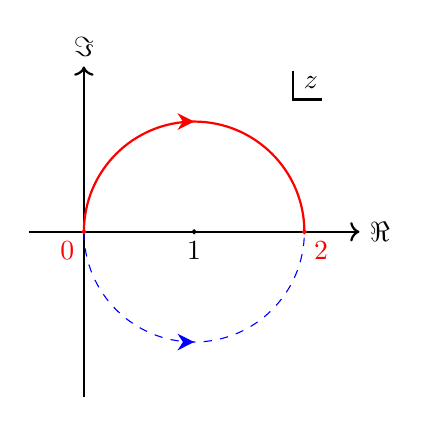
\begin{tikzpicture}[scale=1.4]
  % Axes
  \draw[->,thick] (-0.5,0) -- (2.5,0) node[right] {$\Re$};
  \draw[->,thick] (0,-1.5) -- (0,1.5) node[above] {$\Im$};

  % Arc rouge avec flèche
  \draw[red,thick,mid arrow] 
    (0,0) arc[start angle=180,end angle=0,radius=1];
  \draw[blue,dashed,mid arrow] 
    (0,0) arc[start angle=180,end angle=360,radius=1];

  % Points 0 et 2
  \filldraw[red] (0,0) circle (0.5pt) node[below left] {$0$};
  \filldraw[red] (2,0) circle (0.5pt) node[below right] {$2$};

  \node at (2.06,1.35) {$z$};
\draw[thick] (1.9,1.457) -- (1.9,1.2) -- (2.16,1.2);

  % Centre
  \filldraw (1,0) circle (0.5pt) node[below] {$1$};
\end{tikzpicture}
\end{minipage}
\end{center}
 \caption{Left: \textit{Stable} contour in red \textit{vs} \textit{Unstable} contour in blue. Right: corresponding contours in $z=1+e^{2t}$.}
    \label{fig:contoursfortandz}
\end{figure}
We now specify to the case of a massless scalar field in $d+1=4$ dimensions $(\nu=\frac{d}{2}=\frac{3}{2}~,~\Delta_+^{\text{dS}}=d=3)$. One then finds
\begin{equation}
    \begin{aligned}
         \Phi_n(t)\propto &~ (1+e^{-2t})^{n-1}~\times \Bigg[{}_2F_1\left(\frac{1}{2}+n,n-1,-\frac{1}{2};-e^{-2t}\right)\\
         &+\frac{8}{3}n(n^2-1)(1-z(t))^{-\frac{3}{2}}{}_2F_1\left(2+n,\frac{1}{2}+n,\frac{5}{2};-e^{-2t}\right)\Bigg]~.
    \end{aligned}
\end{equation}
This expresses the expansion of the Euclidean vacuum in terms of Mottola ``in" and ``out" states~\cite{PhysRevD.32.3136,Bousso_2002}. Finally, it remains to choose the appropriate branch for $(1-z(t))^{-\frac{3}{2}}$ depending on the contour. The function being double-valued, there are two non-equivalent class of contours. The standard red contour corresponds to rotating $t=-i\t$. As $t$ runs over this contour (see Fig.~\ref{fig:contoursfortandz}), z describes an upper semi-circle in the positive part of the complex plane. Thus, one picks up a factor of $\exp(-\frac{3}{2}(-i\pi))=-i$. The opposite happens for the other contour. The final solution $\Phi^\star_n$ reads
\begin{equation}
    \begin{aligned}
         \Phi_n^\star(t)= &~ (1+e^{-2t})^{n-1}~\times \Bigg[{}_2F_1\left(\frac{1}{2}+n,n-1,-\frac{1}{2};-e^{-2t}\right)\\
         &\pm i\frac{8}{3}n(n^2-1)e^{-3t}{}_2F_1\left(2+n,\frac{1}{2}+n,\frac{5}{2};-e^{-2t}\right)\Bigg]~.
    \end{aligned}
\end{equation}
In this formula the $-$ sign corresponds to the red contour while the $+$ sign corresponds to the blue contour. From~\eqref{eq:phistar} and \eqref{eq:formulapowerspectrum}, we can directly extract the power spectrum (we re-establish the $H$-dependence)
\begin{equation}\label{eq:power_spectrum_BD}
    \mathcal{P}(n; \infty)=\mp \frac{H^2}{2n(n^2-1)}\,.
\end{equation}
The two analytic continuations yield complex-conjugate perturbative wave functions. The first continuation gives Gaussian-suppressed fluctuations, whereas the opposite continuation gives an inverse Gaussian. Although the latter contour is sometimes associated with a naive path-integral implementation of the tunnelling proposal, it should not automatically be identified with Vilenkin’s original tunnelling wave function. In the Wheeler–DeWitt formulation, the tunnelling boundary condition acts primarily on the homogeneous background branch, while regularity of the perturbative wave function independently selects the de Sitter-invariant vacuum and Gaussian-suppressed fluctuations. The relation between the two descriptions depends on the boundary terms and perturbative boundary conditions used in defining the gravitational path integral. For further details regarding this question, see~\cite{PhysRevD.37.888,Lehners:2023yrj,Vilenkin_2018}.\PG{It seems that in 2017 and 2018, there were lots of conflicts associated to that between Lehners/Vilenkin/Hartog so I don't know anymore what to say about the contour}In what follows, we will thus assume that the chosen contour is the red one such that $t=-i\tau$ with $\tau<0$ in the Euclidean region. We also recover the expected scale invariance of the power spectrum. Indeed,
\begin{equation}\label{eq:dimensionless_power_spectrum_BD}
    \Delta^{\Phi}_{n}=\frac{H^2}{4\pi^2}\,.
\end{equation}

We end this part by noting that in the massless case, the ODE \eqref{eq:EOMPhilor_mode_general_d} admits exact algebraic solutions \cite{Wada:1986uy,Lehners:2023yrj,PhysRevD.37.888}. In particular the regular solution $\Phi^\star_n$ (for $d=3$) reads
\begin{equation}\label{closedform}
    \begin{aligned}
        \Phi^\star_n=\frac{(1+i\,\sinh(Ht))^{\frac{n-1}{2}}(i\sinh(Ht)-n)}{(i\,\sinh(Ht)-1)^{\frac{n+1}{2}}}\,.
    \end{aligned}
\end{equation}
This solution corresponds to damped oscillations, whose number increases with the angular momentum $n$ (see Fig.~\ref{fig:scale_f}). 
\PG{Curiosity: in terms of the variable $v=\sinh(Ht)$, such function has algebraic branch points at $v=\pm i$ if $n$ is even and has a pole of order $(n+1)/2$ if $n$ is odd. Such point is mapped to the south pole.}

We finished this subsection by noting that the $n=1$ lowest mode is singular as the power spectrum diverges for this value. This IR divergence is tied to the global shift symmetry $\Phi \to \Phi +c$ in the massless case.


%%%%%%%%%%%%%%%%%%%%%%%%%%%%%%%%%%%%%%%%%

\begin{figure}[t!]
\begin{center}
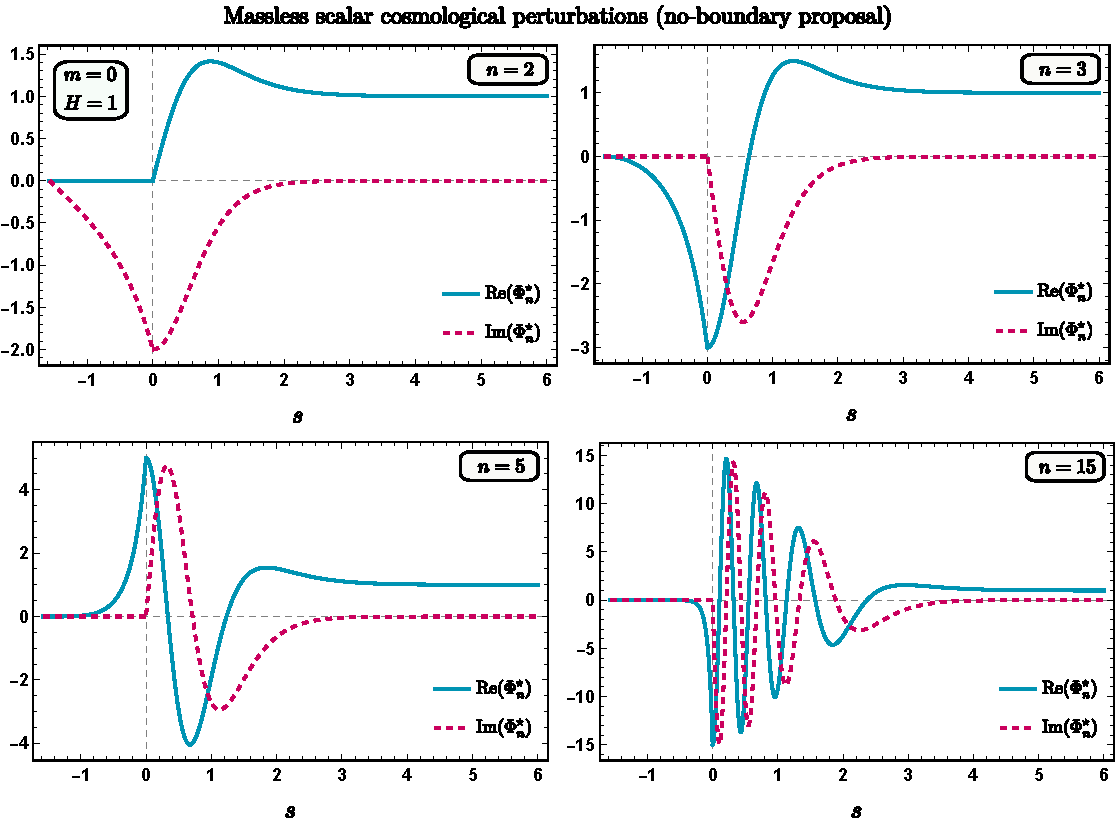
\includegraphics[width=\textwidth]{Figures_paper_2/figure_no_boundary.pdf}
\end{center}
\caption{Massless scalar cosmological perturbations for different angular momenta $n=2,3,5,15$ in the context of the no-boundary proposal. The complex time contour is chosen as $s=\tau$ for $s<0$ and $s=t$ for $s>0$. Parameters used are $m=0$ and $H=1$.\PG{rename $\ell \to n+1$} \IG{Fixed! I did the replacement $\ell \to n-1$.}}
\label{fig:scale_f}
\end{figure}


\subsection{Perturbations in the ``wineglass" wormhole}

%%%%%%%%%%%%%%%%%%%%%%%%%%%%%%%%%%%%%%%%%%%%%%%%%%%%%%%%%%
\section*{Acknowledgments}
P.B. acknowledges financial support from the European Research Council (grant BHHQG-101040024), funded by the European Union.
\\
The work of IDG was supported by the Estonian Research Council grants MOB3JD1202, RVTT3,  RVTT7, and by the CoE program TK202 ``Fundamental Universe''. \\
This article is based upon work from COST Action CA21136 – “Addressing observational tensions in cosmology with systematics and fundamental physics (CosmoVerse)”, supported by COST (European Cooperation in Science and Technology).\\
Views and opinions expressed are those of the authors only and do not necessarily reflect those of the European Union or the European Research Council. Neither the European Union nor the granting authority can be held responsible for them.\\
Finally, IDG wishes to thank the CERN Theoretical Physics Department for hospitality while this research was being carried out.

\appendix

%%%%%%%%%%%%%%%%%%%%%%%%%%%%%%%%%%%%%%%%%%%%%%%%%%%%%%%%%%%%%

\section{Spherical harmonics on the three sphere}\label{harmonics}
Scalar harmonics on the unit three-sphere satisfy\footnote{We adopt the same conventions as Halliwell and Hawking in~\cite{Halliwell:1984eu}.}
\begin{equation}
    \Delta_{S^3}Q_{n\ell m}(\Omega)
    =
    -(n^2-1)Q_{n\ell m}(\Omega)\,, \quad n \in \mathbb{N}^\star,\,\ell \in\{0,...,n-1\},\, |m| \leq\ell
\end{equation}
A convenient construction starts from the factorized complex basis
\begin{equation}
    \mathcal{Q}_{n\ell m}(\chi,\theta,\varphi)
    =
    H_{n\ell}(\chi)Y_{\ell m}(\theta,\varphi),
\end{equation}
where $H_{n\ell}(\chi)$ is real and can be expressed in terms of
Gegenbauer polynomials, while $Y_{\ell m}$ are the usual complex
spherical harmonics on $S^2$. In the standard phase convention,
\begin{equation}
    Y_{\ell m}^{*}
    =
    (-1)^mY_{\ell,-m}\,.
\end{equation}
We then define real spherical harmonics on \(S^2\) by
\begin{equation}
Y_{\ell m}^{\mathrm{R}}
=
\begin{cases}
\displaystyle
Y_{\ell 0},
& m=0,
\\[0.25cm]
\displaystyle
\frac{1}{\sqrt{2}}
\left[
Y_{\ell m}+(-1)^mY_{\ell,-m}
\right],
& m>0,
\\[0.35cm]
\displaystyle
\frac{1}{i\sqrt{2}}
\left[
Y_{\ell |m|}
-
(-1)^{|m|}Y_{\ell,-|m|}
\right],
& m<0.
\end{cases}
\end{equation}
The modes with $m>0$ and $m<0$ are respectively the cosine- and
sine-type real harmonics. A real orthonormal basis of scalar harmonics on $S^3$ is therefore
\begin{equation}
    Q_{n\ell m}(\chi,\theta,\varphi)
    =
    H_{n\ell}(\chi)
    Y_{\ell m}^{\mathrm{R}}(\theta,\varphi).
\end{equation}
A scalar field can consequently be expanded as
\begin{equation}
    \Phi(\tau,\Omega)
    =
    \sum_{n=1}^{\infty}
    \sum_{\ell=0}^{n-1}
    \sum_{m=-\ell}^{\ell}
    \Phi_{n\ell m}(\tau)
    Q_{n\ell m}(\Omega).
\end{equation}
On a real spacetime slice, the reality of the scalar field imposes the reality of the hyperspherical harmonic coefficients $\Phi_{n \ell m}$. The field may nevertheless become complex when analytically continued along the Euclidean-Lorentzian contour.

\section[Analytic matching procedure in the large n limit]{Analytic matching procedure in the large $n$ limit}

\begin{figure}[htb]
\centering
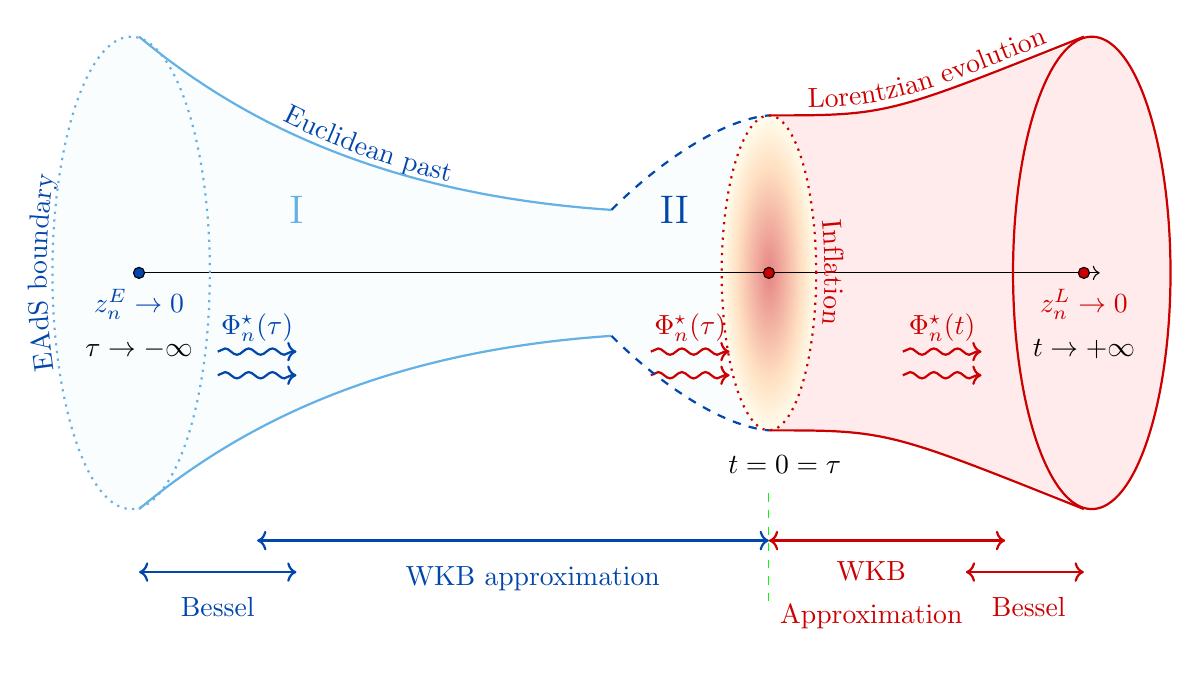
\begin{tikzpicture}


\path[fill=cyan!10, opacity=0.25]
  (-7.1,0)
  arc[start angle=180,end angle=270,x radius=1,y radius=3] 
  .. controls (-4.8,-2) and (-3,-1) .. (0,-0.8)
  .. controls (0.6,-1.4) and (1.4,-1.95) .. (2,-2)     
  arc[start angle=-90,end angle=-270,x radius=0.6,y radius=2]
   % change this angle=270 to  angle=90
  .. controls (1.4,1.95) and (0.6,1.4) .. (0,0.8)
  .. controls (-3,1) and (-4.8,2) .. (-6.1,3)
  arc[start angle=90,end angle=180,x radius=1,y radius=3]
  -- cycle;

\path[fill=red, opacity=0.08]
  (1.4,0)
  arc[start angle=180,end angle=-90,x radius=0.6,y radius=2] 
   % change this angle=-90 to  angle=270
  .. controls (3.5,-2) .. (6.1,-3)                    
  arc[start angle=-90,end angle=90,x radius=1,y radius=3]  
  .. controls (3.5,2) .. (2,2)                        
  arc[start angle=90,end angle=180,x radius=0.6,y radius=2]  
  -- cycle;

% \shade[inner color=red4!60,  outer color=orange!40, opacity=0.6] 
%   (2,0) ellipse (0.6 and 2);

\pgfdeclareradialshading{inflationellipse}{\pgfpoint{0cm}{0cm}}{
  color(0cm)=(red4!80);
  color(0.6cm)=(orange!40);
  color(0.9cm)=(yellow!10)
}
\shade[shading=inflationellipse, opacity=0.6] (2,0) ellipse (0.6 and 2);



% horizontal axis
\draw[->] (-6,0) -- (6.2,0);

% Points
\filldraw[fill=navyblue] (-6,0) circle (2pt) node[below] {$\begin{array}{c} \color{navyblue}{z_n^E \to 0}\\ \tau \to -\infty\end{array}$};
\filldraw[fill=red4] (2,0) circle (2pt);
\filldraw[fill=red4] (6,0) circle (2pt) node[below] {$\begin{array}{c} \color{red4}{z_n^L \to 0} \\ t \to +\infty \end{array}$};


\draw[thick, red4, decorate, 
      decoration={text along path, text={Lorentzian evolution}, text align=center, text color=red4}] 
      (2,2.1) .. controls  (3.5,2.1) .. (6,3.1);
\draw[thick, navyblue, decorate, 
      decoration={text along path, 
                  text={Euclidean past}, 
                  text align=center,
                  text color=navyblue}] 
      (-5.9,3.1) .. controls (-4.8,2.1) and (-3,1.1) .. (0,0.8);
\draw[thick, navyblue, decorate,
      decoration={
      text along path,
                  text={EAdS boundary},
                  text align=center,
                  text color=navyblue, reverse path, raise=3.5pt}
                ] 
       (-6,3) .. controls (-7.4,2.8) and (-7.4,-2.8)  .. (-6,-3);
\draw[thick, red4, decorate,
      decoration={
      text along path,
                  text={Inflation},
                  text align=center,
                  text color=red4
                   ,  raise=3pt
                  }
                ] 
       (2,2) .. controls (2.8,1.8) and (2.8,-1.8)  .. (2,-2);


% Regions
\node[above] at (-4,0.5) {\Large\color{cornflowerblue}{I}};
\node[above] at (0.8,0.5) {\Large\color{navyblue}{II}};


% Legend points
\node[below] at (2.2,-2.2) {$t =0 = \tau$};

% Waves

\draw[->, decorate, decoration={snake, amplitude=0.4mm, segment length=3mm}, thick, navyblue] (-5,-1) -- (-4,-1) node[midway, above] {$\Phi^\star_{n}(\tau)$};
\draw[->, decorate, decoration={snake, amplitude=0.4mm, segment length=3mm}, thick, navyblue] (-5,-1.3) -- (-4,-1.3);


\draw[->, decorate, decoration={snake, amplitude=0.4mm, segment length=3mm}, thick, red4] (0.5,-1) -- (1.5,-1) node[midway, above] {$\Phi^\star_{n}(\tau)$};
\draw[->, decorate, decoration={snake, amplitude=0.4mm, segment length=3mm}, thick, red4] (0.5,-1.3) -- (1.5,-1.3);


\draw[->, decorate, decoration={snake, amplitude=0.4mm, segment length=3mm}, thick, red4] (3.7,-1) -- (4.7,-1) node[midway, above] {$\Phi^\star_{n}(t)$};
\draw[->, decorate, decoration={snake, amplitude=0.4mm, segment length=3mm}, thick, red4] (3.7,-1.3) -- (4.7,-1.3);

\draw[thick, cornflowerblue, dotted] (-6.1,0) ellipse (1 and 3);   %
\draw[thick, red4] (6.1,0) ellipse (1 and 3);   % 
\draw[thick, red4, dotted] (2,0) ellipse (0.6 and 2);

% 
% \draw[thick, navyblue]
%   (-6,3) .. controls (-4.8,2) and (-3,1) .. (0,0.8)
%         .. controls   (0.6,1.4) and (1.4,1.95) .. (2,2);

% \draw[thick, navyblue]
%   (-6,-3) .. controls (-4.8,-2) and (-3,-1) .. (0,-0.8)
%          .. controls (0.6,-1.4) and (1.4,-1.95) ..(2,-2);

\draw[thick, cornflowerblue]
  (-6,3) .. controls (-4.8,2) and (-3,1) .. (0,0.8);

\draw[thick, cornflowerblue]
  (-6,-3) .. controls (-4.8,-2) and (-3,-1) .. (0,-0.8);

% Δεξί (γαλάζιο) κομμάτι
\draw[thick, dashed, navyblue]
  (0,0.8) .. controls (0.6,1.4) and (1.4,1.95) .. (2,2);

\draw[thick, dashed, navyblue]
  (0,-0.8) .. controls (0.6,-1.4) and (1.4,-1.95) .. (2,-2);


\draw[thick, red4] (2,2) .. controls  (3.5,2) .. (6,3);
\draw[thick, red4] (2,-2) .. controls (3.5,-2) .. (6,-3);

\draw[<->,thick, navyblue] (-6,-3.8) -- (-4,-3.8);
\node[below] at (-5,-4) {\color{navyblue} \text{Bessel}};

\draw[<->,thick, navyblue] (-4.5,-3.4) -- (2,-3.4);
\node[below] at (-1,-3.6) {\color{navyblue} \text{WKB approximation}};

\draw[<->,thick, red4] (2,-3.4) -- (5,-3.4);
\node[below] at (3.3,-3.4) {$\begin{array}{c} {\color{red4}\text{WKB}}\\{\color{red4} \text{Approximation}}\end{array}$};

\draw[<->,thick, red4] (4.5,-3.8) -- (6,-3.8);
\node[below] at (5.3,-4) {\color{red4} \text{Bessel}};

\draw[-, dashed, green] (2, -2.8) -- (2, -4.2) ;


\end{tikzpicture}
\caption{Schematic view of the WKB matching problem.}
\label{fig:waves_WKB}
\end{figure}

\subsection{Leading WKB order results}

We divide the half-wineglass wormhole in 4 regions (see Fig.~\ref{fig:waves_WKB}) :
\begin{itemize}
    \item The region near the EAdS boundary $H_{\rm AdS}\tau\to -\infty$ .
    \item An Euclidean region overlapping with the previous region and extending to the junction point $\tau=0=t$ .
    \item A Lorentzian region extending the junction point and overlapping with the asymptotically dS region .
    \item The asymptotically dS region where $H t \to \infty$ .
\end{itemize}
\paragraph{The region near the EAdS boundary $H_{\rm AdS}\tau\to -\infty$ .}\label{par:AdSboundary}
We start defining the variables
\begin{equation}
    k_n := \sqrt{n^2-1}\,, \qquad z_n^{E} :=\frac{k_n}{H_{\rm AdS}\,a}\,.
\end{equation}
After changing the variable from $\tau$ to $z_n^{E}$ in~\eqref{eq:EOMPhieuc_mode}, one obtains the following differential equation for a single mode $\Phi_n$
\begin{equation}\label{eq:interm_Bessel}
    \frac{d^2\Phi_n}{d\left(z_n^{E}\right)^2} \left(z_n^{E}\right)^2 \left(\frac{a'}{a}\right)^2+\frac{d\Phi_n}{dz_n^{E}}\left[-2\left(\frac{a'}{a}\right)^2z_n^{E} - z_n^{E}\frac{\partial }{\partial \tau }\left( \frac{a'}{a}\right)\right]-H^2_{\rm AdS}\left(z_n^{E}\right)^2 \Phi_n =0\,.
\end{equation}
With the ansatz for the scale factor, this is easily seen that 
\begin{equation}
    \frac{a'}{a} \underset{H_{\rm AdS} \tau\to -\infty}{=} -H_{\rm AdS}+ \mathcal{O}\left(e^{2H_{\rm AdS}\tau}\right)\,.
\end{equation}
Note crucially that the subleading terms are independent of $n$. Hence, up to terms of order $\mathcal{O}\left(e^{2H_{\rm AdS}\tau}\right)$,~\eqref{eq:interm_Bessel} reduces to a barely modified Bessel equation
\begin{equation}
     \left(z_n^{E}\right)^2\frac{d^2\Phi_n}{\rm{d}\left(z_n^{E}\right)^2} -2z_n^{E}\frac{d\Phi_n}{dz_n^{E}}-\left(z_n^{E}\right)^2 \Phi_n =0\,.
\end{equation}
The regular solution at the EAdS boundary is of the form 
\begin{equation}
    \Phi_n(z) \propto \left(z_n^{E}\right)^{3/2}I_{3/2}(z_n^{E})\,.
\end{equation}
This solution holds for all $z$ as long as $H_{\rm AdS}\tau\to -\infty$. For latter, it is useful to extract the asymptotic expansion of the regular solution for large $z_n^{E}$ which requires $k_n\gg H_{\rm AdS}a$.  One finds
\begin{equation}\label{eq:largezBessel}
    \Phi_n(z_n^{E})\underset{z\to \infty}{\propto }z_n^{E} e^{z_n^{E}}\,.
\end{equation}
Even better, since we know the complete asymptotic expansion of the Bessel $I_{\nu}$ function, we can write
\begin{equation}\label{eq:asymptotic_expansion_nonperturb}
    \Phi_n(z_n^{E})\underset{z\to \infty}{\propto }z_n^{E} e^{z_n^{E}}+ ... \, + z_n^{E} e^{-z_n^{E}}+ ... \,\,.
\end{equation}
Note that it contains two branches. This will allow us to identify non-perturbative corrections in $k_n$.
\paragraph{Euclidean region overlapping with the previous region and extending to the junction point $\tau=0=t$ .}
We now look for an approximate WKB solution. We first rewrite the equation in Schrödinger form using the ansatz $\Phi_n(\tau)=a^{-3/2}\psi_n(\tau)$. It yields
\begin{equation}\label{eq:WKB_euclidean_beforeturning}
    \psi''_n(\tau)-\left[\frac{3}{4}\left(\frac{a'}{a}\right)^2+\frac{3}{2}\frac{a''}{a}+\frac{k_n^2}{a^2}\right]\psi_n(\tau)=0\,.
\end{equation}
Suppose $k_n\gg1$. Then, it is clear from the previous equation, that in the central region of the wormhole the two first terms can be neglected. Upon this assumption, we can neglect the two first terms of the Schrödinger potential in this approximation. The two independent leading WKB estimates are of the form
\begin{equation}\label{eq:WKB_sol_euclidean_before_turning}
    \Phi^{\text{WKB},\textbf{E}}_{n,\pm}(\tau) = \frac{1}{a(\tau)}\exp\left[\pm k_n \int_{-\infty}^{\tau}\frac{\rm{d}\tau'}{a(\tau')} \right]\,.
\end{equation}
The WKB approximation is then valid as long as $\frac{a'}{k_n}\ll1$. This is obviously true in the central region. This also holds in the asymptotic EAdS region for which $|a'|\sim H_{\rm AdS} a $ provided $k_n\gg a H_{\rm AdS}$. Given these assumptions, there exists an overlap with the previous region defined by the condition
\begin{equation}
    1\ll z_n^E \ll k_n\,.
\end{equation}
The first ensures the validity of the WKB approximation while the second ensures the validity of the Bessel ansatz since $k_n /  z_n^E = a H_{\rm AdS}\gg 1 \Longleftrightarrow H_{\rm AdS}\tau \to -\infty$. We also learn that the overlap region only exists for large $k_n$. Matching~\eqref{eq:largezBessel} with~\eqref{eq:WKB_sol_euclidean_before_turning} in the overlap region selects that a regular solution is proportional to $\Phi_{n,+}^{\text{WKB},\textbf{I}}(\tau)+\Phi_{n,-}^{\text{WKB},\textbf{I}}(\tau)$ at leading order. We introduce the Eikonal integral
\begin{equation}
    \Theta^E_n :=k_n \int_{-\infty}^{0}\frac{\rm{d}\tau'}{a(\tau')}\,.
\end{equation}
The value of the regular solution $\Phi_n^\star$ and its derivative at $\tau=0$ is then
\begin{equation}
    \Phi_n^\star(0) = \mathcal{N}_n \frac{\exp(\Theta^E_n)+\exp(-\Theta_n^E)}{a_0}\,,\quad \frac{\rm{d}\Phi_n^{\star}}{\rm{d}\tau}(0) = \mathcal{N}_n \frac{k_n\left(\exp(\Theta^E_n)-\exp(-\Theta_n^E)\right)}{a_0^{2}}\,,
\end{equation}
where $\mathcal{N}_n$ is a complex normalization constant.

\paragraph{Lorentzian region extending to the junction point and overlapping with the asymptotically dS region .}
Here again the validity of the WKB approximation is the same condition as previously stated but with $H$ replaced by $H_{\rm AdS}$. Hovewer, because of the Lorentzian evolution, the two branches are oscillatory. The leading WKB estimates are of the form
\begin{equation}\label{eq:WKB_Lorentzian}
    \Phi^{\text{WKB},\textbf{L}}_{n,\pm}(t) = \frac{1}{a(t)}\exp\left[\pm i k_n \int_{t}^{\infty}\frac{\rm{d}t'}{a(t')} \right]\,.
\end{equation}
We define the Eikonal integral
\begin{equation}
    \Theta^L_n :=k_n \int_{0}^{\infty}\frac{\rm{d}t'}{a(t')}\,,
\end{equation}
and we have 
\begin{equation}
    \Phi^{\text{WKB},\textbf{L}}_{n,\pm}(0) = \frac{\exp(\pm i \Theta^L_n)}{a_0}\,, \quad \frac{\rm{d}\Phi^{\text{WKB},\textbf{L}}_{n,\pm}}{\rm{d} t}(0)= \frac{\mp i k_n \exp(\pm i \Theta^L_n)}{a_0^{2}}\,.
\end{equation}
$\Phi_n^\star$ should be a linear combination of these two WKB estimates
\begin{equation}
    \Phi_n^\star(t) = A_{n,+} \Phi^{\text{WKB},\textbf{L}}_{n,+}(t) + A_{n,-} \Phi^{\text{WKB},\textbf{L}}_{n,-}(t)\,,
\end{equation}
and we find 
\begin{equation}
    \begin{aligned}
        A_{n,+} &= \mathcal{N}_n \exp(-\Theta_n^E-i\Theta_n^L)\,, \\
        A_{n,-} &= \mathcal{N}_n \exp(\Theta_n^E+i\Theta_n^L)\,,
    \end{aligned}
\end{equation}
by imposing the gluing condition at $t=0=\tau$~\eqref{eq:gluing_condition} with $t=-i\tau$. $\left|\frac{A_{n,+}}{A_{n,-}}\right| = e^{-2\Theta_n^E}\ll1$ is exponentially small. In this sense, incorporating the $+$ will generate non-perturbative corrections. 

\paragraph{The asymptotically dS region where $H t \to \infty$ .}
This again parallels the situation described in~\ref{par:AdSboundary} but with $z_n^E$ replaced by $z_n^L := \frac{k_n}{a H}$. The effective equation for $\Phi_n$ now reduces to a Bessel type of equation
\begin{equation}
     \left(z_n^{L}\right)^2\frac{d^2\Phi_n}{\rm{d}\left(z_n^{L}\right)^2} -2z_n^{L}\frac{d\Phi_n}{dz_n^{L}}+\left(z_n^{L}\right)^2 \Phi_n =0\,.
\end{equation}
Indeed, let $\Phi_n := \left(z_n^{L}\right)^{3/2}\chi_n$. $\chi_n$ obeys a Bessel equation with parameter $\nu = 3/2$. There are two relevant basis. The first one corresponds to the Hankel Basis $H^{\pm}_\nu$. Because of the asymptotic properties of the Hankel functions for large argument 
\begin{equation}
    H_\nu^\pm(z) \sim \sqrt{\frac{2}{\pi z}} \exp\left[\pm i\left(z-\frac{\nu \pi}{2} -\frac{\pi}{4}\right)\right]\,,
\end{equation}
this makes it clear that in the overlap region
\begin{equation}
    1 \ll z_n^L \ll k_n\,,
\end{equation}
The WKB estimates are proportional to the Hankel solutions. Precisely, we find
\begin{equation}\label{eq:BesselsHWKB}
    \Phi^{\text{WKB},\textbf{L}}_{n,\pm} = -\frac{H}{k_n}\sqrt{\frac{\pi}{2}} \left(z_n^L\right)^{3/2}H^{\pm}_{3/2}(z_n^L)\,.
\end{equation}
The second basis corresponds to Bessel functions of the first kind $J_{\pm3/2}$. Such basis is well adapted to describe the constant and decaying branches in the asymptotically dS region. Indeed, in this region, we have $(z_n^L)^{3/2}J_{-3/2}(z_n^L) \propto \text{const}$ and $(z_n^L)^{3/2}J_{3/2}(z_n^L)\propto e^{-3 H t}$. Recalling \eqref{eq:phistar}, we can express $\Phi_n^\star(t)$ in terms of the Bessel functions of the first kind (this matches the conventions defined in~\eqref{eq:leadingbehavior_massless},~\eqref{eq:ansatzs_scalefactor} and \eqref{eq:phistar})
\begin{equation}
    \Phi_n^\star = \sqrt{\frac{\pi}{2}}\left(z_n^L\right)^{3/2}\left[ -J_{-3/2}(z_n^L)+ \Gamma_n \times \frac{3\alpha^3}{8k_n^3}\,J_{3/2}(z_n^L)\right]\,.
\end{equation}
Using~\eqref{eq:BesselsHWKB}, we also have
\begin{equation}
\begin{aligned}
        \Phi_n^\star &= -\mathcal{N}_n \exp\left(\Theta_n^E+i\Theta_n^L\right) \frac{H}{k_n}\sqrt{\frac{\pi}{2}}(z_n^L)^{3/2}H^-_{3/2}(z_n^L)\\
        &-\mathcal{N}_n \exp\left(-\Theta_n^E-i\Theta_n^L\right) \frac{H}{k_n}\sqrt{\frac{\pi}{2}}(z_n^L)^{3/2}H^+_{3/2}(z_n^L)
        \,.
\end{aligned}
\end{equation}
Using the connections formulas relating the Hankel functiona to the standard Bessel basis, we easily find the values of $\mathcal{N}_n$ and $\Gamma_n$ to be
\begin{equation}\label{eq:GammaleadingWKB}
    \mathcal{N}_n = -i\frac{k_n}{2H}\frac{1}{\sinh\left[-\Theta_n^E-i\Theta_n^L\right]}\,, \quad \Gamma_n = -i\frac{8 k_n^3}{3\alpha^3}\,.
\end{equation}
The power spectrum can be deduced from~\eqref{eq:GammaleadingWKB} and~\eqref{eq:formulapowerspectrum} and is found to be
\begin{equation}
    \mathcal{P}^{WG}(n) = \frac{H^2}{2k_n^3}=\mathcal{P}_{N.B}(n)\left(1+\frac{1}{n^2}\right) \,.
\end{equation}
\PG{Even this formula Panos tells you that there should be perturbative corrections...}
We conclude that for large $n$ the power spectrum is the same as in the no-boundary proposal. This is a universal feature which is independent of the precise details of the geometry.
\paragraph{Comment in the choice of contour}
Note that the implementation of the gluing condition corresponds to the stable contour. Here again, there are two different sets of contours (the one that we discussed in the stable one). The reason is the algebraic branch point of the Bessel $I_{3/2}$ at $z=0$ which corresponds to the EAdS boundary.

\subsection{Perturbative connection matrix and higher order WKB}

\PG{It does not seem to be so easy to find higher order corrections...}

Consider $\tilde{R}_n(\tau)= \frac{\Phi_n'}{\Phi_n}$ (this is the counterpart in the Euclidean region to the variable defined before~\eqref{eq:Riccati_equation_Lor}). This variables solves a simple Riccati equation
\begin{equation}\label{eq:Riccati_euclidean}
    \tilde{R}_n' + 3\frac{a'}{a}\tilde{R}_n + \tilde{R}_n^2 = \frac{k_n^2}{a^2}\,.
\end{equation}
This can be exploited to find the corrections to the leading order WKB method. Assume that $\tilde{R}_n$ is given by a power series in $k_n$
\begin{equation}
    \tilde{R}_n = k_n \tilde{R}^{(1)} + \tilde{R}^{(0)} + \frac{\tilde{R}^{(-1)}}{k_n} + \mathcal{O}\left(\frac{1}{k^2_n}\right)\,.
\end{equation}
This yields a differential-difference equation for the coefficients
\begin{equation}
\begin{cases}
     \left(\tilde{R}^{(1)}\right)^2 = \frac{1}{a^2} \,,
     \\[0.3cm]
     \tilde{R}^{(-p+1)} + 3 \frac{a'}{a}\tilde{R}^{(-p+1)} + \sum_{i+j=p-1} \tilde{R}^{(-i)}\tilde{R}^{(-j)}= 0\,, \quad p\geq0\,.
\end{cases}
\end{equation}
The initial value $\tilde{R}^{(1)}$ yields the two WKB branches described previously at leading order. This is then immediate to find
\begin{equation}
    \tilde{R}_{n,\pm}(\tau) = \pm\frac{k_n}{a} - \frac{a'}{a}\pm\frac{1}{k_n}\left[\frac{a''}{2}+\frac{a'^2}{2a}\right] + \mathcal{O}\left(\frac{1}{k_n^2}\right)\,.
\end{equation}
The corresponding WKB estimate can be obtained by a simple integration and it is clear that the two first terms gives back~\eqref{eq:WKB_sol_euclidean_before_turning}. 
One can check that the logarithmic derivative of $(z_n^E)^{3/2}I_{3/2}(z_n^E)$ with respect to $\tau$ exactly matches the expansion of $\tilde{R}_{n,+}$.
One can play the same game in the Lorentzian region for the Riccati variable $R_n = \frac{\partial_t \Phi^\star_n}{\Phi^\star_n}$ finding (with conventions that matches~\eqref{eq:WKB_Lorentzian})
\begin{equation}
    R_{n,\pm}(t) = \mp i\frac{k_n}{a}-\frac{\dot{a}}{a} \pm \frac{i}{k_n}\left[\frac{a''}{2}+\frac{a'^2}{2a}\right]+ \mathcal{O}\left(\frac{1}{k_n^2}\right)\,.
\end{equation}
Since $R_n$ solves a first order equation, it suffices to match the value at $t=\tau=0$. If the $+$-branch is selected in Euclidean, it is straightforward to check that (stable contour)
\begin{equation}\label{eq:branch_exchange}
    R_{n,+}(0) = i \tilde{R}_{n,-}(0)
\end{equation}
This statement (provided smoothness of the scale factor(which is not true in our case) is valid to all orders in perturbation theory! The question is where are supposed to come perturbative connections? Since, we saw that to all order in perturbation theory, the exchange of branch is valid~\eqref{eq:branch_exchange}, it should come from the Bessel-WKB matching (near EAdS and in the asymptotically dS region) will lead to a mixture of the $\pm$ branches. Note also that even if in the Euclidean region, we have $\Phi_n^\star\propto \Phi_{n,+}+b_n \Phi_{n,-}$ in any case we would have 
\begin{equation}
    A_{n,+} = \mathcal{N}_n b_n \exp(-\Theta_n^E-i\Theta_n^L) \ll A_{n,-}
\end{equation}
if $b_n$ is not exponentially large. Thus, the $-$ Lorentzian branch will inevitably be selected at the perturbative level. I conclude that corrections should come from some kind of Stokes phenomenon in the asymptotically dS region. I checked the resurgence series of $H_{\nu}$ see https://dlmf.nist.gov/10.17 an in particular (10.17.17). Curiously, observe that for $\nu = 3/2$, there is no resurgence!  I thus conclude that the perturbative corrections should come by perturbing the dS Bessel equation by including corrections from the scale factor. These corrections will bring back resurgence and allow mixture of the branches.

\section{Numerical procedure}
\PG{I will add my github repository so that the code is accessible to anyone. I'll also add a note on the code so that everything is comprehensible.}
In order to obtain the power spectrum, the formula~\eqref{eq:power_spectrum_1} shows that it suffices to extract the late time behaviour of the Riccati variable $\mathcal{W}_n$ solving~\eqref{eq:Riccati_W} in order to obtain the power spectrum. The steps are the following
\begin{itemize}
    \item Step \textbf{1}: Impose the boundary condition at the Euclidean endpoint of the contour.
    \item Step \textbf{2}: Obtain the value of the Riccati variable at the gluing point $t=\tau=0$ by numerically integrating the equation of motion in euclidean time $\tau = i t$ up to $\tau=0$.
    \item Step \textbf{3}: Use this value at initial condition to run the equation of motion in Lorentzian time.
    \item Step \textbf{4}: Extract the late-time behavior $t \gg \frac{1}{H} $ to obtain the power spectrum.
\end{itemize}
We implemented the code in Python. It is available on the following github repo together with a note added on how to run it. Such a code can be used for any pre-inflationnary models specified by the form of the scale factor.

\subsection{No-boundary proposal}
Before discussing the case of the wineglass wormhole, it is instructive to work out the case of the no-boundary proposal. This serves as a benchmark example for which we know the exact results concerning the power-spectrum in the Bunch-Davies vacuum~\eqref{eq:power_spectrum_BD},\,\eqref{eq:dimensionless_power_spectrum_BD}.

Step \textbf{1}: The regular solution at the south pole behaves as $\sim \left(\tau + \frac{ \pi}{2}\right)^{n-1}$. In practice, we take $\tau_{\rm ini} = -\frac{\pi}{2H}+\delta$ with $\delta \ll 1$ and impose
\begin{equation}
    \mathcal{W}_n(\tau_{\rm ini}) = \frac{H(n-1)}{\delta} a^3(\tau_{\rm ini})\,.
\end{equation}

Step \textbf{2}: We numerically integrate from $\tau_{\rm ini}$ to $\tau=0$ 
\begin{equation}
    \mathcal{W}_n'(\tau) = a(n^2-1) - \frac{\mathcal{W}_n^2}{a^3}\,.
\end{equation}
and extract the value $\mathcal{W}_n(0)$.

Step \textbf{3}: We numerically integrate from $t=0$ to $t_f\gg \frac{1}{H}$ the equation of motion for $\mathcal{W}_n$ in Lorentzian time~\eqref{eq:Riccati_W}
\begin{equation}
    \dot{\mathcal{W}_n}= i \left[a(n^2-1)-\frac{\mathcal{W}_n^3}{a^2}\right]\,.
\end{equation}

Step \textbf{4}: Extract the power spectrum from $\mathcal{W}_n(t_f)$ using~\eqref{eq:power_spectrum_1}.

We display the comparaison between the exact analytical results and the numerical results concerning the dimensionless power spectrum.

\begin{figure}[htb]
    \centering
    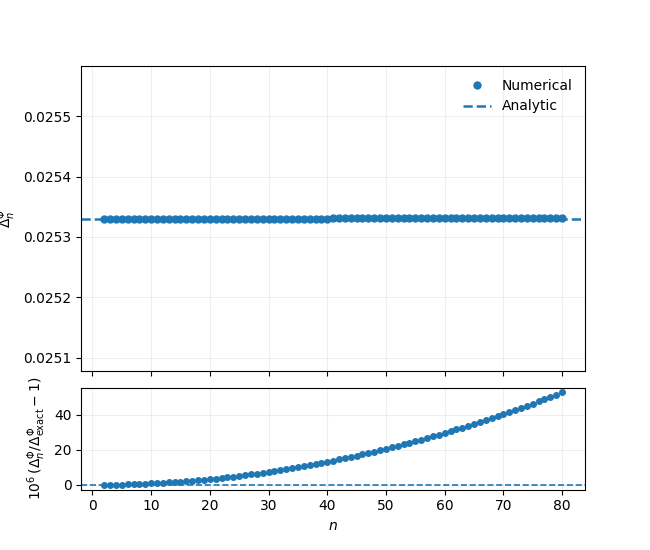
\includegraphics[width=0.8\linewidth]{Figures_paper_2/noboundarycomparaison.png}
    \caption{We compare analytic exact results~\eqref{eq:dimensionless_power_spectrum_BD} compared to numerical results concerning the dimensionless power spectrum for the first $80$ harmonics. The numerical algorithm used $H=1,\,\delta = 10^{-4},\,t_f = 10 H = 10$. As can be seen in the lower panel, the relative discrepancy grows with $n$  and is smaller than $10^{-4}$.}
    \label{fig:comparaisonnoboundary}
\end{figure}

\subsection{Wineglass proposal}
We have to go through the same steps.

Step \textbf{1}: The regularity condition is imposed at the EAdS boundary which in $\tau$ coordinates is at $\tau=-\infty$. The regular solution at the EAdS boundary behaves as $\sim e^{3H_{I}\tau}$. In practice, this is better to first compactify this direction by introducing $u(\tau) = \exp(2H_{I}(\tau-\tau_{\rm min}))$ ($\tau = -\infty$ is mapped to $u=0$ while $\tau_{\rm min}$ is mapped to $u=1$). We thus impose
\begin{equation}
    \mathcal{W}_n(\delta) = 3 H_I \,a^3(\tau(\delta))\,.
\end{equation}

Step \textbf{2}: The Euclidean evolution is divided into two regions and the scale factor is only $C^3$. In order to obtain the Euclidean portion of the solution, we numerically integrate region \textbf{I} ( $\tau <\tau_{\rm min}$) imposing the previous initial condition and then integrate in region \textbf{II} using continuity at $\tau_{\rm min}$ to impose the new initial boundary condition.

The following steps go exactly as in the case of the no-boundary proposal. We display the comparison between the wineglass power spectrum and the Bunch-Davies power spectrum.

\begin{figure}[htb]
    \centering
    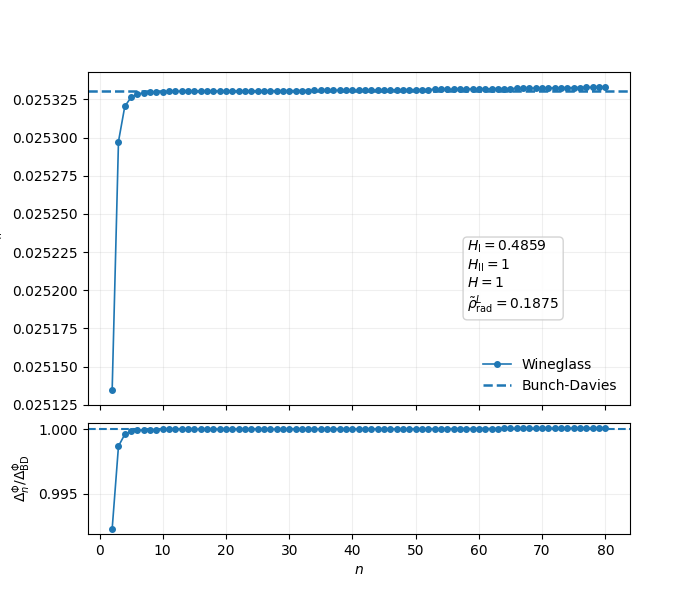
\includegraphics[width=0.8\linewidth]{Figures_paper_2/new80harmonics.png}
    \caption{We compare the Bunch-Davies power spectrum~\eqref{eq:dimensionless_power_spectrum_BD} to numerical results concerning the dimensionless power spectrum for the first $80$ harmonics. The numerical algorithm used $H=1,\,\delta = 10^{-4},\,t_f = 10 H = 10\,,\, H_{\rm II} =1  $.}
    \label{fig:comparaisonnoboundary_w_80_H_II_1}
\end{figure}

\begin{figure}[htb]
    \centering
    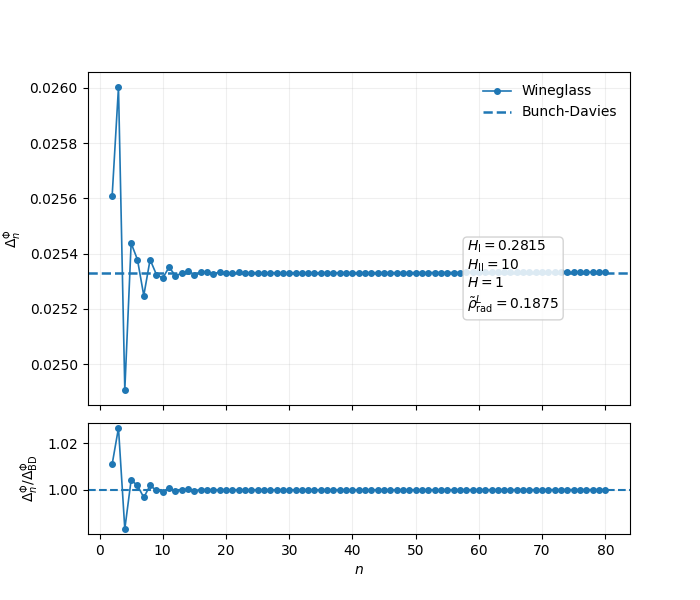
\includegraphics[width=0.8\linewidth]{Figures_paper_2/newnew80harmonics.png}
    \caption{We compare the Bunch-Davies power spectrum~\eqref{eq:dimensionless_power_spectrum_BD} to numerical results concerning the dimensionless power spectrum for the first $80$ harmonics. The numerical algorithm used $H=1,\,\delta = 10^{-4},\,t_f = 10 H = 10\,,\, H_{\rm II} =10  $.\PG{As can be seen the inverse radius of EAdS or equivalently the Hubble size of the wormhole neck $\sim1/H_{\rm II}$ has a large influence on the power spectrum. For smaller Hubble size of the wormhole neck, the lower harmonics get more affected. This is sort of expected.  }}
    \label{fig:comparaisonnoboundary_w_80_H_II_10}
\end{figure}

\subsection{Discrepancy with the Bunch-Davies vacuum at the start of inflation.}
\paragraph{First possibility: we impose that the radius of dS region is the same and compute the discrepancy even though the radius at the origin is not the same!}
The discrepancy with respect to the Bunch-Davies vacuum is nicely captured by the variable
\begin{equation}
    \frac{\Delta \mathcal{W}_n}{\mathcal{W}_n}\Bigg|_{t=0} := \frac{\mathcal{W}_n(t)-\mathcal{W}^{BD}_n(t)}{\mathcal{W}_n(t)}\Bigg|_{t=0} = \frac{\mathcal{W}_n(0)-a_0^2\frac{n^2-1}{n}}{\mathcal{W}_n(0)}=\frac{\mathcal{W}_n(0)-\frac{n^2-1}{nH_{\rm NB}^2}}{\mathcal{W}_n(0)}\,.
\end{equation}
For the wineglass and the no-boundary complex saddles to asymptote to the same universe, this requires to fix the Hubble radius as a function of the radiation energy density of the wineglass so that we should substitute the value of $H_{\rm NB}^2$ for $\tilde{\rho}^L_{\rm rad}$ in the previous expression (see~\eqref{eq:Lorentzian_wineglass})
\begin{equation}
    \frac{\Delta \mathcal{W}_n}{\mathcal{W}_n}\Bigg|_{t=0} = \frac{\mathcal{W}_n(0)-16\frac{n^2-1}{3n \tilde{\rho}^L_{\rm rad}}}{\mathcal{W}_n(0)}\,.
\end{equation}
We then fix the inverse radius of the EAdS region $H_{\rm I}$ and plot such quantity as a function of $n$ for different value of the radiation energy density $\tilde{\rho}^L_{\rm rad}$.

\begin{figure}[htb]
    \centering
    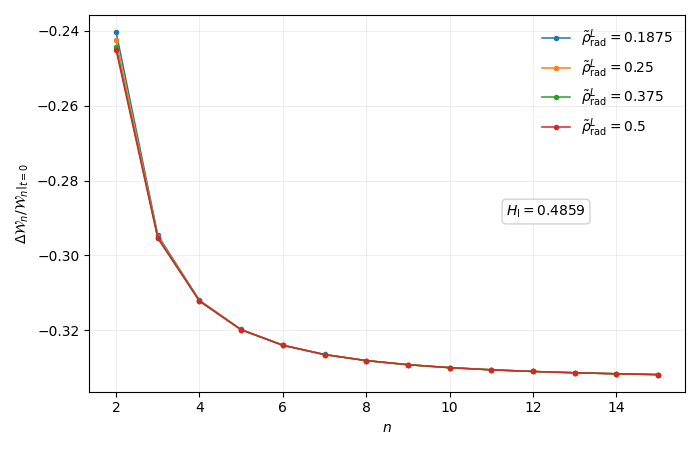
\includegraphics[width=0.8\linewidth]{Figures_paper_2/discrepancyasymptoticallydS.png}
    \caption{We compare the Riccati variables at the onset of inflation by imposing that they asymptote to the same universe with the same Hubble radius. The numerical algorithm used $\,\delta = 10^{-4},\,t_f = 10 H = 10\,,\, H_{\rm II} =1  $.}
    \label{fig:comparaisonnoboundary_w_Riccati_0H_II_1}
\end{figure}


\begin{figure}[htb]
    \centering
    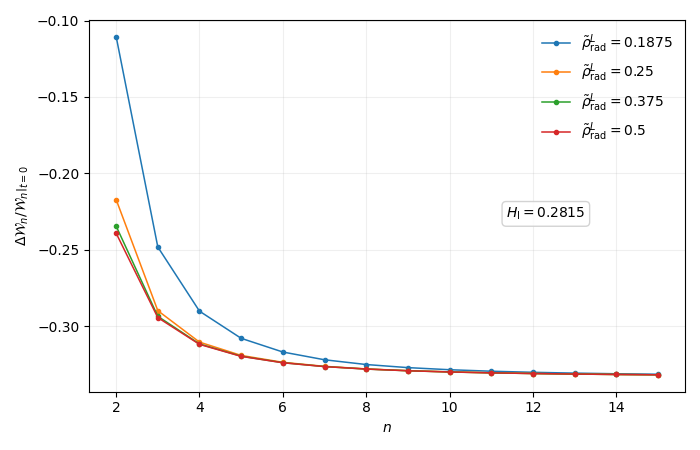
\includegraphics[width=0.8\linewidth]{Figures_paper_2/discrepancyasymptoticallydStwo.png}
    \caption{We compare the Riccati variables at the onset of inflation by imposing that they asymptote to the same universe with the same Hubble radius. The numerical algorithm used $\,\delta = 10^{-4},\,t_f = 10 H = 10\,,\, H_{\rm II} =10  $.}
    \label{fig:comparaisonnoboundary_w_Riccati_0H_II_10}
\end{figure}


\paragraph{Second possibility: we impose that they have the same radius at the onset of inflation}
This means that we shall tune $a_0$ in the previous formula such that $a^2_0 = (a_0^{H-WG})^2 = \frac{3}{4H_{WG}^2} = 4\tilde{\rho}^L_{\rm rad}$ and thus
\begin{equation}
    \frac{\Delta \mathcal{W}_n}{\mathcal{W}_n}\Bigg|_{t=0} = \frac{\mathcal{W}_n(0)-4\tilde{\rho}^L_{\rm rad}\frac{n^2-1}{n}}{\mathcal{W}_n(0)}\,.
\end{equation}

\begin{figure}[htb]
    \centering
    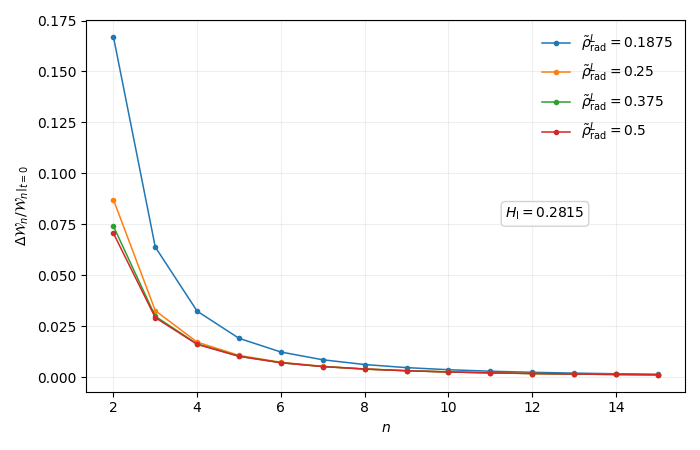
\includegraphics[width=0.8\linewidth]{Figures_paper_2/discrepancyonsetinflation.png}
    \caption{We compare the Riccati variables at the onset of inflation by imposing that the size of the transverse slices is the same at $t=0$. The numerical algorithm used $\,\delta = 10^{-4},\,t_f = 10 H = 10\,,\, H_{\rm II} =10  $.\PG{As you can see, this plot reproduces Lehners results which is expected given the way they compute things...}}
    \label{fig:comparaisonnoboundary_w_Riccati_0H_II_10_Lehners}
\end{figure}

\section{Minisuperspace Wheeler-DeWitt wavefunction in Einstein-scalar theory}
Consider a Einstein theory with a minimally coupled scalar field
\begin{equation}
    \mathcal{S}_L = \int \rm{d}^4 x \sqrt{-g} \left(\frac{\mathcal{R}}{2\kappa}-\frac{1}{2}\left(\partial_\mu\phi\right)^2 -V(\phi)\right)\,.
\end{equation}
We consider truncating the quantum gravity theory to minisuperspace metrics
\begin{equation}
    \rm{d}s^2 = -N^2(t)\rm{d}t^2 + a^2(t)\rm{d}\Omega_3^2\,,\quad \phi =\phi(t)\,,
\end{equation}
where $N$ denotes the lapse function incorporating the possibility of time-reparametrization. After computing the Ricci scalar curvature and performing basic algebra the Lorentzian action is found to be
\begin{equation}
    \mathcal{S}_L = 2\pi^2 \int \rm{d}t \left\{\frac{3}{\kappa}\left[aN -\frac{a \dot{a}^2}{N} \right]+\frac{a^3 \dot{\phi}^2}{2N}-Na^3 V(\phi)\right\}\,.
\end{equation}
The conformal mode problem is visible in that the kinetic term of the scale factor comes with the opposite sign to that of the scalar field kinetic term. To simplify notations, we introduce $\tilde{\phi}=\sqrt{\kappa/3} \,\phi,\,\tilde{V}(\tilde{\phi}) = \frac{\kappa}{3}V(\phi)$ so that
\begin{equation}
    \mathcal{S}_L = \frac{6\pi^2}{\kappa}\int \rm{d}t \left[aN -\frac{a \dot{a}^2}{N} +\frac{a^3 \dot{\tilde{\phi}}^2}{2N}-Na^3 \tilde{V}(\tilde{\phi})\right]\,.
\end{equation}
We now define the symplectic structure and derive the corresponding Hamiltonian. The ``position" variables are taken to be $(a,\tilde{\phi})$ and the corresponding conjugate momenta are found to be
\begin{equation}
    \pi_a :=\frac{\delta \mathcal{S}_L}{\delta \dot{a}}= -\frac{6\pi^2}{\kappa}\frac{2\dot{a}a}{N}\,, \quad \pi_{\tilde{\phi}}:=\frac{\delta \mathcal{S}_L}{\delta \dot{\tilde{\phi}}} = \frac{6\pi^2}{\kappa}\frac{a^3\dot{\tilde{\phi}}}{N}\,.
\end{equation}
Performing the Legendre transform of the Lagrangian associated to $\mathcal{S}_L$, the Hamiltonian is found to be
\begin{equation}
    \mathcal{H} = N\frac{\kappa}{6\pi^2}\left[-\frac{\pi_a^2}{4a}+\frac{\pi_{\tilde{\phi}}^2}{2a^3} - \left(\frac{6\pi^2}{\kappa}\right)^2 \left(a-a^3\tilde{V}(\tilde{\phi})\right)\right]\,.
\end{equation}
The lapse function appears as a Lagrangian multiplier thus encapsulating the gauge invariance. Canonical quantization proceeds standardly by turning the``position" variables and conjugate momenta to operators on the Hilbert space and the Poisson brackets are turned into commutators with a factor of $i$. In ``position" space, the action of the conjugate momenta becomes simply $-i\frac{\partial}{\partial q}$ for each position variable $q$. The Wheeler-DeWitt constraint is the statement that physical states $\Psi(\tilde{\phi},a)$ should be annihilated by the Hamiltonian, generator of time-reparametrization. At this stage an operator-ordering ambiguity arises, since the scale factor $a$ does not commute with its conjugate momentum. In the case where the minisuperspace is one dimensional (in absence of $\phi$), this operator-ordering ambiguity is in one to one correspondence with the path-integral choice of measure and so on the inner product structure for which the Hamiltonian is Hermitian. For further discussions and resolutions of this subtle point, see~\cite{Kaimakkamis:2024lkb}. In what follows, we will simply discard these subtleties since we are interesting in the semi-classical WKB-wavefunction and the semi-classical WKB wavefunction is insensitive to normal ordering ambiguities~\cite{Vilenkin:1987kf}. A simple example is the case where $\pi_a$ directly acts on the wavefunction
\begin{equation}\label{eq:WdWfinal}
    \left[\frac{\partial^2}{\partial a^2}-\frac{2}{a^2}\frac{\partial^2}{\partial \tilde{\phi}^2}-\left(\frac{12\pi^2}{\kappa}a\right)^2 \left(1-a^2\tilde{V}(\tilde{\phi})\right)\right]\Psi(\tilde{\phi},a)=0\,.
\end{equation}
We may further assume that the potential satisfies $a^2 V \ll M^2_{pl}\Rightarrow a^2 \tilde{V} \ll 1$ and is slowly varying $\tilde{V}(\tilde{\phi}) = H^2$. We thus neglect derivatives with respect to $\tilde{\phi}$ at firstobtaining a one-dimensional minisuperspace Wheeler-DeWitt equation
\begin{equation}
    \left[\frac{\partial^2}{\partial a^2}-\left(\frac{12\pi^2}{\kappa}a\right)^2 \left(1-a^2 H^2\right)\right]\Psi(a)=0\,.
\end{equation}
The effective potential of the equation is $U(a) = \left(\frac{12\pi^2}{\kappa}a\right)^2 \left(1-a^2H^2\right)$. There are two regions. If $aH>1$, the potential is negative and this corresponds to the classically allowed region. The two WKB estimates are therefore
\begin{equation}
    \Psi^{(1)}_{\pm}(a) = \exp\left[\pm i\int_{H^{-1}}^a \rm{d} \tilde{a}\sqrt{-U(\tilde{a})}\right] = \exp\left[\pm i\frac{4\pi^2}{\kappa H^2}\left((aH)^2-1\right)^{3/2}\right]\,.
\end{equation}
In the classically forbidden region $aH<1$, the two WKB estimates are 
\begin{equation}
    \Psi^{(2)}_{\pm}(a) = \exp\left[\pm\int_{a}^{H^{-1}} \rm{d}\tilde{a}\sqrt{U(\tilde{a})}~ \mp i\frac{\pi}{4}\right] = \exp\left[\pm\frac{4\pi^2}{\kappa H^2}(1-a^2H^2)^{3/2}~ \mp i\frac{\pi}{4}\right]\,.
\end{equation}
Now, we discuss the different proposals for the choice of the WKB wavefunction. The Hartle-Hawking proposal selects the growing branch in the classically forbidden region ($aH<1$)
\begin{equation}
    \Psi_{HH}(a) \propto \Psi_-^{(2)}(a)=\exp\left[-\frac{4\pi^2}{\kappa H^2}(1-a^2H^2)^{3/2}+i\frac{\pi}{4}\right]\,.
\end{equation}
The WKB connection formulae then gives in the classically allowed region
\begin{equation}
     \Psi_{HH}(a)\propto\cos\left[\left((aH)^2-1\right)^{3/2}-\frac{\pi}{4}\right]\,.
\end{equation}
The Tunneling proposal consists in selecting only outgoing modes in the classically allowed region
\begin{equation}
    \Psi_{T}(a)  \propto \exp\left(-\frac{4\pi^2}{\kappa H^2}\left[1+i\left((aH)^2-1\right)^{3/2}\right]\right)\,.
\end{equation}
In the classically allowed region, the Tunneling wavefunction is then found to be 
\begin{equation}
    \Psi_{T}(a)  \propto \Psi_+^{(2)}(a)-\frac{i}{2}\Psi_-^{(2)}(a)\,.
\end{equation}



The overall normalization may be discussed by re-establishing the dependence on $\tilde{\phi}$~\cite{halliwell2009introductorylecturesquantumcosmology}. We first illustrate such procedure for the Hartle-Hawking wavefunction. Observe that neglecting such a depencence is only valid for non-vanishing $a$ as the coefficient in front of the $\tilde{\phi}$ second-derivative explodes. We write the wavefunction (in the classically forbidden region) as
\begin{equation}
    \Psi_{\rm HH}(a,\tilde{\phi}) = A(\tilde{\phi})\exp\left[-\frac{4\pi^2}{\kappa \tilde{V}(\tilde{\phi})}\left(1-a^2 \tilde{V}(\tilde{\phi})^{3/2}\right)\right]\,.
\end{equation}
Taking the derivative with respect to $\tilde{\phi}$ and then taking the $a\to 0$ limit, we obtain that the zero flux condition imposes\footnote{The neglected terms in the second derivative will be of order $\mathcal{O}(a^2)$ so that the limit $a \to 0$ is actually $0$ for the potential problematic term in~\eqref{eq:WdWfinal}.}
\begin{equation}
    \frac{\rm{d}A}{\rm{d}\tilde{\phi}}+A(\tilde{\phi})\frac{4\pi^2}{\kappa\tilde{V}^2(\tilde{\phi})}\frac{\rm{d}\tilde{V}}{\rm{d}\tilde{\phi}} =0 \Rightarrow A(\tilde{\phi}) \propto \exp\left[\frac{4\pi^2}{\kappa \tilde{V}(\tilde{\phi})}\right] \,.
\end{equation}

% \section{Fuchsian equations: recipe}
% \subsection{Hypergeometric functions}\label{hypergeo}

% \paragraph{General solution to the massive scalar differential equation in the no-boundary geometry.} Our starting point is equation ... . To bring it into a hypergeometric form, we need to eliminate one order for each pole appearing in the third coefficient. To achieve that, we use the ansatze 
% \[
% \begin{aligned}
%     \Phi_n(z)=z^{\beta}(z-1)^{\alpha}\varphi_\ell(z)~.
% \end{aligned}
% \]
% The equation for $\varphi_\ell$ reads
% \begin{align*}
%         \varphi_\ell''+&\varphi_\ell'\left[\frac{2\alpha}{z-1}+\frac{2\beta}{z}+\frac{1}{z-1}\left(\frac{d+2}{2}-\frac{d}{z}\right)\right]+\varphi_\ell\times \frac{N(z)}{z^2(z-1)^2}=0~,
% \end{align*}
% where primes correspond to derivatives with respect to $z$ and  
% \[
% \begin{aligned}
%     N(z)&=z(z-1)\left[\alpha(\alpha-1)+\beta(\beta-1)+2\alpha\beta+\frac{d+2}{2}\beta+\frac{d+2}{2}\alpha+\frac{m^2}{4}\right]\\
%     &+z\left[\alpha(\alpha-\frac{d}{2})-\beta(\beta+d-1)+\ell(\ell+d-1)+\frac{m^2}{4}\right]\\
%     &+\beta(\beta+d-1)-\ell(\ell+d-1)~.
% \end{aligned}
% \]
% Here we factorized the leading coefficient by $z(z-1)$ as we wish to cancel one order of each pole appearing in the third coefficient of the equation for $\varphi_\ell$. Thus, we shall choose $\alpha$ and $\beta$ such that the term in $z^1$ and $z^0$ vanish in the expression of $N(z)$. Clearly, $\beta=\ell$ and we also have
% \[
% \begin{aligned}
%     &\alpha^2-\alpha\frac{d}{2}+\frac{m^2}{4}=0\Rightarrow \alpha_{\pm}=\frac{1}{2}\Delta_{\pm}^{dS}~.\\
%     &\text{with}~~\Delta_{\pm}^{dS}=\frac{d}{2}\pm\mu=\frac{d}{2} \pm \sqrt{\frac{d^2}{4}-m^2}
% \end{aligned}
% \]
% Then one can extract the hypergeometric parameters comparing to the hypergeometric equation to find
% \begin{align*}
%         &a=\ell+\frac{d}{2}~,\quad b=\ell+\frac{d}{2}+\mu~,\quad c=2\ell+d~.
% \end{align*}

% Thus, the regular solution at $z=0$ reads
% \begin{equation}
%     \Phi_n(z) \propto (z-1)^{\frac{1}{2}\Delta_+^{\text{dS}}}z^l \times F(\ell+\frac{d}{2},\ell+\frac{d}{2}+\mu,2\ell+d;z)~,
% \end{equation}
% This is exactly the result given in \cite{Maldacena:2024uhs}.

% \paragraph{Connection formula relating the regular solution at $0$ to the basis at $z=\infty$.}
% \begin{equation}\label{otoinfhypergeo}
%     \begin{aligned}
%     F(a,b,c;z)&=\frac{\Gamma(c)\Gamma(b-a)}{\Gamma(b)\Gamma(c-a)}(1-z)^{-a}F\left(a,c-b,a-b+1;\frac{1}{1-z}\right)\\
%     &+\frac{\Gamma(c)\Gamma(a-b)}{\Gamma(a)\Gamma(c-b)}(1-z)^{-b}F\left(b,c-a,b-a+1;\frac{1}{1-z}\right)~.
%     \end{aligned}
% \end{equation}

% \paragraph{No-boundary proposal: basis $\Phi_\pm$ at $t\rightarrow\infty$.}

% Focusing on the massless case, $\Phi_\pm$ are exactly given by
% \begin{equation}\label{closedformsnobound}
%     \begin{aligned}
%         &\Phi_-(t)=\left(1+e^{-2t}\right)^{\ell}F\left(\frac{3}{2}+\ell,\ell,-\frac{1}{2};-e^{-2t}\right)~,\\
%         &\Phi_+(t)=\left(1+e^{-2t}\right)^{\ell}\,e^{-3t}\,F\left(3+\ell,\frac{3}{2}+\ell,\frac{5}{2};-e^{-2t}\right)~.
%     \end{aligned}
% \end{equation}


% \subsection{Heun functions}\label{Heuneq}

% Heun equation was first introduced in 1889 by Karl M. W. L. Heun. It consists in a Fuchsian differential equation of order 2 with 4 regular singularities. 
% \begin{equation}\label{Heeunform}
% \frac{d^2\varphi}{dz^2}+\left(\frac{c}{z}+\frac{d}{z-1}+\frac{e}{z-f}\right)\frac{d\varphi}{dz}+\frac{\alpha\beta z-q}{z(z-1)(z-f)}\varphi=0~.
% \end{equation}
% $f,~c,~d,~e,~\alpha,~\beta,~q$ are Heun parameters. In addition we have the identity : $\alpha+\beta+1=c+d+e$. The singularities are at $0,~1,~f,~\infty$. Heun parameters are related to the characteristic  exponents around each regular singularity. Precisely, respectively around $0,1,f,\infty$, the indicial exponents are $\{0,1-c\},~\{0,1-d\},~\{0,1-e\},~\{\alpha,\beta\}$. 
% The regular solution around $0$ is denoted by  $\text{HeunG}[f,\,q,\,\alpha,\,\beta,\,c,d\,;\,z]$.

% \paragraph{Basis of solutions near each regular singularity.}

% \begin{itemize}
%     \item \textbf{Around 0}
% \end{itemize}
% \[
% \begin{aligned}
%     &\varphi_-^{(0)}=\text{HeunG}[f,\,q,\,\alpha,\,\beta,\,c,\,d;\,z]\\
%     &\varphi_+^{(0)}=z^{1-c}~\text{HeunG}[f,\,q-(c-1)(fd+e),\,\alpha+1-c,\,\beta+1-c,\,2-c,\,d;\,z]
% \end{aligned}
% \]

% \begin{itemize}
%     \item \textbf{Around 1}
% \end{itemize}
% \[
% \begin{aligned}
%     &\varphi_-^{(1)}=\Big(\frac{z-f}{1-f}\Big)^{-\alpha}~\text{HeunG}\Big[f,\,q+\alpha(d-\beta),\,\alpha,\,c+d-\beta,\,d,\,c;\,f\frac{1-z}{f-z}\Big]\\
%     &
%     \begin{multlined}
%         \varphi_+^{(1)}=\Big(\frac{z-f}{1-f}\Big)^{-\alpha-1+d}(1-z)^{1-d}~\text{HeunG}\Big[f,\,q-\alpha(\beta+d-2)+(d-1)(\alpha+\beta-1-fc),\,\\
%         \alpha+1-d,\,1+c-\beta,\,2-d,\,c;\,f\frac{1-z}{f-z}\Big]
%     \end{multlined}
% \end{aligned}
% \]

% \begin{itemize}
%     \item \textbf{Around $f$}
% \end{itemize}
% \[
% \begin{aligned}
%     &\varphi_-^{(f)}=\text{HeunG}\Big[\frac{f}{f-1},\,\frac{q-f\alpha\beta}{1-f},\,\alpha,\,\beta,\,e,\,d,\,\frac{z-f}{1-f}\Big]\\
%     &
%     \begin{multlined}
%         \varphi_+^{(f)}=(f-z)^{1-e}~\text{HeunG}\Big[\frac{f}{f-1},\,\frac{q-f\alpha\beta}{1-f}-(e-1)\left(\frac{f}{f-1}d+c\right),\,\\
%         \alpha+1-e,\,\beta+1-e,\,2-e,\,d;\,\frac{z-f}{1-f}\Big]
%     \end{multlined}
% \end{aligned}
% \]

% \begin{itemize}
%     \item \textbf{Around $\infty$}
% \end{itemize}
% \[
% \begin{aligned}
%     &\varphi_+^{(\infty)}=z^{-\alpha}~\text{HeunG}\Big[f,\,q-\alpha\beta(1+f)+\alpha(d+fe),\,\alpha,\,\alpha-c+1,\,\alpha-\beta+1,\,\alpha+\beta+1-c-d;\,\frac{f}{z}\Big]\\
%     &
%     \varphi_-^{(\infty)}=z^{-\beta}~\text{HeunG}\Big[f,\,q-\alpha\beta(1+f)+\beta(d+fe),\,\beta,\,\beta-c+1,\,\beta-\alpha+1,\,\alpha+\beta+1-c-d;\,\frac{f}{z}\Big]
% \end{aligned}
% \]
% \paragraph{Solving the Heun equation for scalar perturbations}\label{Heunequation}

% We start by ... defining tensor perturbations in region ... . We make the change of variable $z=\frac{1+v}{2}$ which will shift the singularity from $-1$ to $0$. The singularities are now at located $0,1,f=\frac{1-(\epsilon-2)}{2}=\frac{3-\epsilon}{2},\infty$.

% \begin{equation}\label{Tensorz'withoutcancelation1}
%     \frac{d^2\Phi_n}{dz^2}+\Big(\frac{3}{z-f}+\frac{z-\frac{1}{2}}{z(z-1)}\Big)\frac{d\Phi_n}{dz}-\frac{m^2(z-f)^2+\frac{1}{4}(n^2-1)}{z(z-1)(z-f)^2}\Phi_n=0~.
% \end{equation}
% Note that in this equation all the singularities are real and the contour described by $z$ in region \textbf{I} is over the real axis and do not pass through any singularity on $(\infty,1)$. Hence, if you impose that $\Phi$ is real at the boundary of EAdS it will remain real up to $z=1$. As you can observe, it matches the form of the Heun equation except for the second order pole in the coefficient of the term without derivative. Hence, we make a power transformation $\Phi_n(z)=(z-f)^{\lambda}\varphi_\ell(z)$ and wish to find an appropriate value for $\lambda$ to cancel one power.
% \begin{equation}\label{varphiequation}
%     \begin{aligned}
%         \varphi_\ell'' 
%     + \varphi_\ell'\left[ \frac{2\lambda}{z-f} + \frac{3}{z-f} + \frac{z - \frac{1}{2}}{z(z-1)} \right]+\varphi_\ell\times \frac{N(z)}{z(z-1)(z-f)^2}=0~.
%     \end{aligned}
% \end{equation}
% where the expression of $N(z)$ is given by
% \begin{align}
%     N(z) &= (z - f) 
%     \left[ (\lambda^2 + 2\lambda)(z + f - 1) 
%     + \lambda\left(z - \frac{1}{2}\right) 
%      - \frac{m^2}{H^2}(z - f) \right] \nonumber
%     \\
%     & - \frac{1}{4}(n^2-1) + f(f - 1)(\lambda^2 + 2\lambda)\,.
% \end{align}
% Thus, we shall choose $\lambda$ such that $-(n^2-1)+4f(f-1)(\lambda^2+2\lambda)=0$. For $\ell$ large, $\lambda$ is complex. We get two possible choices for $\lambda$
% \[
% \lambda_{\pm}=-1\pm i \left(\frac{1}{4f(1-f)}(n^2-1)-1\right)^{1/2}~.
% \]
% From now on, $\lambda$ denotes a solution of the preceding equation. We can now rewrite equation \eqref{varphiequation}

% \begin{equation}\label{HeunI1}
%     \varphi_\ell''+\varphi_\ell'\left[\frac{2\lambda+3}{z-f}+\frac{1/2}{z}+\frac{1/2}{z-1}\right]+\varphi_\ell\times \frac{(\lambda^2+2\lambda)(z+f-1)+\lambda(z-\frac{1}{2})-m^2(z-f)}{z(z-1)(z-f)}=0~.
% \end{equation}
% We are now ready to extract Heun's parameters recalling the form \eqref{Heeunform}
% \[
% c=1/2 , \quad d=1/2, \quad e=2\lambda+3~.
% \]
% Concerning the third term we obtain

% \[
% (\lambda^2+2\lambda)(z+f-1)+\lambda(z-\frac{1}{2})-m^2(z-f)=z\left(\lambda^2+3\lambda-m^2\right)-\left(-m^2f+\frac{\lambda}{2}-\frac{1}{4f}(n^2-1)\right)~,
% \]
% where we used $\lambda^2+2\lambda=\frac{1}{4f(f-1)}(n^2-1)$. Thus
% \[
% q=-m^2f+\frac{\lambda}{2}-\frac{1}{4f}(n^2-1), \quad \alpha \beta=\lambda^2+3\lambda-m^2 \quad \alpha+\beta=c+d+e-1~.
% \]
% $\alpha,~\beta$ can be computed from the two last equations. Introducing the conformal dimensions $\Delta_{\pm}=\frac{d}{2}\pm\sqrt{\frac{d^2}{4}+m^2}$ with $d=3$, one finds
% \[
% \begin{aligned}
% \alpha=\lambda+\Delta_-~, \quad \beta=\lambda+\Delta_+~, \quad q=-m^2f+\frac{\lambda}{2}-\frac{1}{4f}(n^2-1)~.
% \end{aligned}
% \]
% One can check that $\alpha,\beta$ gives the correct asymptotics near the EAdS boundary $z\rightarrow\infty$. Precisely, combining with the prefactor $(z-f)^{\lambda}$, we obtain for the two asymptotic solutions

% \begin{equation}\label{asymptotics}
%     (z^{\lambda-\alpha},z^{\lambda-\beta})=(z^{-\Delta_-},z^{-\Delta_+})~, \quad z\sim e^{-H\tau}~.
% \end{equation}
% Finally, we recall the relation between $z$ and $\tau$, $\Phi$ and $\varphi$

% \[
% \begin{aligned}
% z(\tau)=\frac{1+\cosh(\tau-\tau_{min})}{2}~, \quad \Phi_n(z)=(z-f)^{\lambda}\varphi_\ell(z)~.
% \end{aligned}
% \]
% In region \textbf{III}, the same procedure applies providing the replacements. One finds

% \begin{equation}\label{secondset}
%     \begin{aligned}
%     & \lambda'_{\pm}=-1\pm i\left(\frac{1}{\color{red}4f'(1-f')}(n^2-1)-1\right)^{1/2}~, \quad c'=1/2~, \quad d'=1/2~, \quad e'=2\lambda'+3~,\\
%     &\alpha' =\lambda'+\Delta_-^{dS}~, \quad \beta' =\lambda'+\Delta_+^{dS}~, \quad q'=m^2f'+\frac{\lambda'}{2}+\frac{1}{4f'}(n^2-1)~,
% \end{aligned}
% \end{equation}
% where we defined $\Delta_{\pm}^{dS}=\frac{d}{2}\pm\sqrt{\frac{d^2}{4}-m^2}$. Finally, we recall the relation between $z'$ and $t$,$\Phi$ and $\varphi$

% \[
% \begin{aligned}
% z'(t)=\frac{1+\cosh(t)}{2}=\frac{1+\cos(\tau)}{2}~, \quad \Phi_n(z')=(z'-f')^{\lambda'}\varphi_\ell(z')~.
% \end{aligned}
% \]

% \section{Expansion near the EAdS boundary and at late Lorentzian times}\label{expansion}
% \paragraph{Near boundary expansion}
% Our starting point is \eqref{EOMPhieuc} which we study in the massless limit
% \begin{equation}\label{EOMPhieuclnomass}
%     \Phi_n''(\tau)+3\frac{a'}{a}\,\Phi_n'(\tau)
%   -\frac{(n^2-1)}{a^2}\Phi_n(\tau)=0~.
% \end{equation}
% Recall that the boundary of EAdS corresponds to $\tau\to -\infty$ and $a(\tau)=\frac{e^{-(\tau-\tau_{min})}}{2}+\mathcal{O}(1)$. To simplify notations we call $\tilde{\tau}=\tau-\tau_{min}$ and drop the tildes in what follows. To make contact with the vocabulary of AdS/CFT holography, we introduce $\Delta_-=0,~\Delta_+=d=3$ the corresponding conformal dimensions of the source and the vev. Let's first study the non-renormalizable (source) solution in the massless limit
% \begin{equation}
%     \Phi_-(\tau)=e^{\Delta_-\tau}+a_1\,e^{(\Delta_-+1)\tau}+a_2\,e^{(\Delta_-+2)\tau}+\mathcal{O}(e^{\Delta_+\tau})=1+a_1\,e^{\tau}+a_2\,e^{2\tau}+\mathcal{O}(e^{\Delta_+\tau})~,
% \end{equation}
% where at order $\Delta_+$ log terms appear only for even $d$ signaling the presence of a gravitational conformal anomaly \cite{deHaro:2000vlm}\cite{Henningson:1998gx}.
% Expanding up to order $e^{2\tau}$ equation \eqref{EOMPhieuclnomass}, one obtains
% \begin{equation}
%     \Phi_-(\tau)=1-2(n^2-1)e^{2\tau}+\mathcal{O}(e^{\Delta_+\tau})~.
% \end{equation}
% Such expansion is independent on the precise structure of the wineglass wormhole. Concerning the sub-leading solution $\Phi_+$, the terms appearing in the expansion depend on the details of the throat of the wormhole. In the Euclidean region the scale factor reads (see equation \eqref{eq:scale_ans_m})
% \begin{equation}
%     a(\tau)=\frac{e^{-\tau}}{2}+\epsilon-2+\mathcal{O}(e^{\tau})~.
% \end{equation}
% If we write 
% \begin{equation}
%     \Phi_+(\tau)=e^{\Delta_+\tau}+b_1\,e^{(\Delta_++1)\tau}+\mathcal{O}(e^{(\Delta_++2)\tau})=e^{3\tau}+b_1\,e^{4\tau}+\mathcal{O}(e^{5t})~,
% \end{equation}
% and inject the expansion in \eqref{EOMPhieuclnomass} one finds $b_1=\frac{9\,(2-\epsilon)}{4}$. 

% \paragraph{Expansion at late Lorentzian times}\label{lateLor} In the Lorentzian region, for massless scalar field the equation for cosmological perturbations reads (see \eqref{EOMPhilor})
% \begin{equation}\label{EOMPhilornomass}         
% \ddot{\Phi}_\ell(t)+3\frac{\dot{a}}{a}\,\dot{\Phi}_\ell(t)
%   +\frac{(n^2-1)}{a^2}\Phi_n(t)=0~.
% \end{equation}
% The equation is similar to \eqref{EOMPhieuclnomass} up to a change of sign in the third term. Hence, the asymptotic form of the leading $\Phi_-(t)$ and sub-leading $\Phi_+(t)$ solutions can be obtained from the previous discussion
% \begin{equation}\label{LateLorexp}
% \begin{aligned}
%     &\Phi_-(t)=1+2\ell (\ell+2)e^{-2t}+\mathcal{O}\left(e^{-3t}\right)~,\\
%     &\Phi_+(t)=e^{-3t}+\tilde{b_1}\,e^{-4t}+\mathcal{O}\left(e^{-5t}\right)~.
% \end{aligned}
% \end{equation}
% The term $\tilde{b_1}$ is depends on the background geometry considered. One finds
% \begin{equation}\label{auxilaryparam}
%     \tilde{b_1} = 
%     \begin{cases}
%    \displaystyle   0\, \quad  \text{No-boundary geometry}
% \\[0.4cm]
%    \displaystyle \frac{9\,\epsilon}{4}~ \,\text{Wineglass wormhole}\,.
%     \end{cases}
% \end{equation}











%%%%%%%%%%%%%%%%%%%%%%%%%%%%%%%%%%%%%%%%%%%%%%%%%%%%%%%%%%%%%
\bibliographystyle{JHEP}
\bibliography{biblio}

\end{document}



















% ============================================================
% LEFT PANEL
% ============================================================
\begin{subfigure}[c]{0.40\textwidth}
\centering

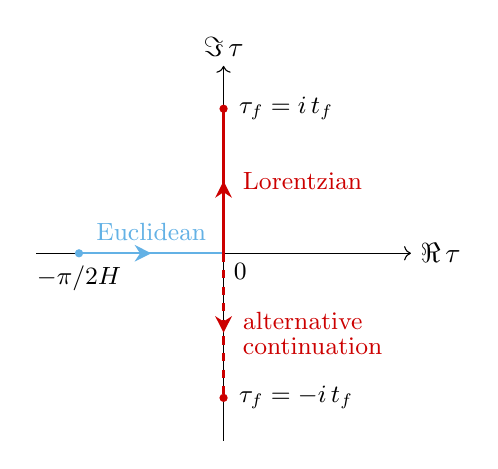
\begin{tikzpicture}[
    scale=0.68,
    mid arrow/.style={
        postaction={
            decorate,
            decoration={
                markings,
                mark=at position 0.5 with
                {\arrow{Stealth[length=6pt,width=6pt]}}
            }
        }
    },
    upper arrow/.style={
        postaction={
            decorate,
            decoration={
                markings,
                mark=at position 0.32 with
                {\arrow{Stealth[length=6pt,width=6pt]}}
            }
        }
    }
]

\pgfdeclareradialshading{inflationellipse}{\pgfpoint{0cm}{0cm}}{
  color(0cm)=(red4!80);
  color(0.6cm)=(orange!40);
  color(0.9cm)=(yellow!10)
}

% Axes
\draw[->] (-3.5,0) -- (3.5,0)
node[right] {$\Re\,\tau$};

\draw[->] (0,-3.5) -- (0,3.5)
node[above] {$\Im\,\tau$};

% Euclidean contour
\draw[thick,cornflowerblue,mid arrow]
(-2.7,0) -- (0,0);

% Upper Lorentzian contour
\draw[thick,red4,mid arrow]
(0,0) -- (0,2.7);

% Alternative Lorentzian contour
\draw[thick, red4,dashed,postaction={decorate, decoration={ markings, mark=at position 0.55 with  {\arrow{Stealth[length=6pt,width=6pt]}} } } ]
(0,0) -- (0,-2.7);

% Initial point
\fill[cornflowerblue] (-2.7,0) circle (2.2pt);

\node[below=6pt] at (-2.7,0.25)
{\small $-\pi/2H$};

% Upper final point
\fill[red4] (0,2.7) circle (2.2pt);
\node[right=6pt] at (-0.2,2.7)
{\small $\tau_f=i\,t_f$};

% Lower final point
\fill[red4] (0,-2.7) circle (2.2pt);
\node[right=6pt] at (-0.2,-2.7)
{\small $\tau_f=-i\,t_f$};

% Origin label
\node[below right=5pt] at (-0.25,0.25)
{\small $0$};

% Labels
\node[cornflowerblue] at (-1.35,0.40)
{\small Euclidean};

\node[red4,right] at (0.18,1.35)
{\small Lorentzian};

\node[red4,right,align=left] at (0.18,-1.50)
{\small alternative\\[-1mm]\small continuation};

\end{tikzpicture}
\end{subfigure}
\hfill